% Pengaturan ukuran teks dan bentuk halaman dua sisi
\documentclass[10pt,twoside]{report}

% Pengaturan ukuran halaman dan margin
\usepackage[a5paper,top=25mm,left=25mm,right=20mm,bottom=25mm]{geometry}

% Pengaturan ukuran spasi
\usepackage[singlespacing]{setspace}

% Judul dokumen
\title{Buku Laporan Kerja Praktik ITS}
\author{Musk, Elon Reeve \and Kjellberg, Felix Arvid Ulf}

% Pengaturan format bahasa
\usepackage[indonesian]{babel}

% Pengaturan detail pada file PDF
\usepackage[pdfauthor={\@author},bookmarksnumbered,pdfborder={0 0 0}]{hyperref}

% Pengaturan jenis karakter
\usepackage[utf8]{inputenc}

% Pengaturan ukuran indentasi paragraf
\setlength{\parindent}{2em}

% Pengaturan ukuran spasi paragraf
\setlength{\parskip}{0.5ex}

% Package lainnya
\usepackage{etoolbox} % Mengubah fungsi default
\usepackage{enumitem} % Pembuatan list
\usepackage{lipsum} % Pembuatan template kalimat
\usepackage{graphicx} % Input gambar
\usepackage{longtable} % Pembuatan tabel
\usepackage[table,xcdraw]{xcolor} % Pewarnaan tabel
\usepackage[numbers]{natbib} % Kutipan artikel
\usepackage{eso-pic} % Pembuatan background
\usepackage{changepage} % Pembuatan teks kolom
\usepackage{wrapfig} % Wrapping gambar
\usepackage{multirow}
\usepackage{tabularx}
\usepackage{array}
\usepackage{float}
\usepackage[T1]{fontenc} % Memperbaiki masalah tanda kutip dan karakter spesial
\usepackage{textcomp}    % Mendukung simbol tambahan


\usepackage{tikz}
\usetikzlibrary{shapes.geometric, arrows.meta, positioning}

% Pengaturan gaya kotak diagram yang lebih lebar
\tikzstyle{startstop} = [rectangle, rounded corners, minimum width=8cm, minimum height=0.8cm, text centered, draw=black, fill=red!20]
\tikzstyle{process} = [rectangle, minimum width=9cm, minimum height=1cm, text centered, text width=8.5cm, draw=black, fill=orange!20]
\tikzstyle{arrow} = [thick,->,>=stealth]

\tikzstyle{dbteam} = [rectangle, minimum width=9cm, minimum height=1cm, text centered, text width=8.5cm, draw=black, fill=gray!20]
\tikzstyle{author} = [rectangle, minimum width=9cm, minimum height=1cm, text centered, text width=8.5cm, draw=black, fill=cyan!30]
\tikzstyle{arrow} = [thick,->,>=stealth]

% Definisi untuk "Hati ini sengaja dikosongkan"
\def\kosong{
  \thispagestyle{empty}      % Menghilangkan nomor halaman agar tidak terlihat
  \addtocounter{page}{-1}    % Mengurangi hitungan halaman (agar tidak bertambah)
  \vspace*{\fill}
  \begin{center}\textit{Halaman ini sengaja dikosongkan}\end{center}
  \vfill
}
\patchcmd{\cleardoublepage}{\hbox{}}{\kosong}{}{}

% Pengaturan penomoran halaman
\usepackage{fancyhdr}
\fancyhf{}
\renewcommand{\headrulewidth}{0pt}
\pagestyle{fancy}
\fancyfoot[CE,CO]{\thepage}
\patchcmd{\chapter}{plain}{fancy}{}{}
\patchcmd{\chapter}{empty}{plain}{}{}

% Pengaturan format judul bab
\usepackage{titlesec}
\titleformat{\chapter}[display]{\bfseries\Large}{BAB \centering\Roman{chapter}}{0ex}{\vspace{0ex}\centering}[\vspace{2ex}]
\titleformat{\section}{\bfseries\large}{\MakeUppercase{\thesection}}{1ex}{}
\titleformat{\subsection}{\bfseries\large}{\MakeUppercase{\thesubsection}}{1ex}{}
\titleformat{\subsubsection}{\bfseries\large}{\MakeUppercase{\thesubsubsection}}{1ex}{}
\titlespacing{\chapter}{0ex}{0ex}{2ex}
\titlespacing{\section}{0ex}{2ex}{1ex}
\titlespacing{\subsection}{0ex}{1ex}{0.5ex}
\titlespacing{\subsubsection}{0ex}{1ex}{0.5ex}

% Pengaturan persamaan
\newenvironment{conditions}
{\par\vspace{\abovedisplayskip}\noindent
  \tabularx{\columnwidth}{>{$}l<{$} @{${}={}$} >{\raggedright\arraybackslash}X}}
{\endtabularx\par\vspace{\belowdisplayskip}}

% Pengaturan format baris program
\usepackage{listings}
\definecolor{comment}{RGB}{0,128,0}
\definecolor{string}{RGB}{255,0,0}
\definecolor{keyword}{RGB}{0,0,255}
\lstdefinestyle{codestyle}{
  commentstyle=\color{comment},
  stringstyle=\color{string},
  keywordstyle=\color{keyword},
  basicstyle=\footnotesize\ttfamily,
  numbers=left,
  numberstyle=\tiny,
  numbersep=5pt,
  frame=lines,
  breaklines=true,
  prebreak=\raisebox{0ex}[0ex][0ex]{\ensuremath{\hookleftarrow}},
  showstringspaces=false,
  upquote=true,
  tabsize=2,
}
\lstset{style=codestyle}

% Definisi Bahasa JavaScript untuk listings
\lstdefinelanguage{JavaScript}{
  keywords={break, case, catch, continue, debugger, default, delete, do, else, false, finally, for, function, if, in, instanceof, new, null, return, switch, this, throw, true, try, typeof, var, void, while, with},
  morecomment=[l]{//},
  morecomment=[s]{/*}{*/},
  morestring=[b]',
  morestring=[b]",
  ndkeywords={class, export, boolean, throw, implements, import, this},
  keywordstyle=\color{blue}\bfseries,
  ndkeywordstyle=\color{darkgray}\bfseries,
  identifierstyle=\color{black},
  sensitive=false,
  commentstyle=\color{comment}\ttfamily,
  stringstyle=\color{string}\ttfamily,
}



% Isi keseluruhan dokumen
\begin{document}

  % Nomor halaman pembuka dimulai dari sini
  \pagenumbering{roman}

  % Sampul luar
  \input{sampul/sampul-luar.tex}
  \cleardoublepage

  % Sampul dalam
  \thispagestyle{empty}      % Menghilangkan nomor halaman agar tidak terlihat

\AddToShipoutPictureBG*{
  \AtPageLowerLeft{
    % Ubah nilai berikut jika posisi horizontal background tidak sesuai
    \hspace{-3.5mm}

    % Ubah nilai berikut jika posisi vertikal background tidak sesuai
    \raisebox{0mm}{
      
\includegraphics[width=\paperwidth,height=\paperheight]{sampul/sampul-dalam.png}
    }
  }
}

% Pengaturan margin untuk menyesuaikan konten sampul
\newgeometry{top=70mm,left=20mm,right=25mm,bottom=25mm}

\begin{flushleft}

  % Pengaturan jenis teks yang digunakan
  \sffamily

  % Ubah penomoran buku berikut sesuai dengan yang ditentukan oleh departemen
  \noindent\textbf{MAGANG}
  \vspace{6ex}

  % Ubah kalimat berikut sesuai dengan nama perusahaan tempat kerja praktik
  \noindent{\textbf{BADAN PENDAPATAN DAERAH KOTA SURABAYA}} \\
  % Ubah tanggal berikut sesuai dengan waktu berlangsungnya kerja praktik
  \textbf{(7 Juli 2025 -- 15 Agustus 2025)}
  \vspace{6ex}

  % Ubah kalimat berikut sesuai dengan judul topik kerja praktik
  \noindent{\large \textbf{PENGEMBANGAN SISTEM MONITORING PENDAPATAN DAERAH (MonPD Reborn) BERBASIS .NET}}
  \vspace{6ex}

  \begin{adjustwidth}{-2mm}{}
    \begin{tabular}{lcp{0.7\linewidth}}
      % Ubah kalimat-kalimat berikut sesuai dengan nama dan NRP mahasiswa pertama
      \textbf{Azaria Putri Fawnia} & & \textbf{NRP 5024 22 1038} \\
    \end{tabular}
  \end{adjustwidth}
  \vspace{4ex}

  \noindent\textbf{Dosen Pembimbing} \\
  % Ubah kalimat berikut sesuai dengan nama dosen pembimbing
  \textbf{Dr. Arief Kurniawan, S.T., M.T.}
  \vspace{10ex}

  % Ubah kalimat berikut sesuai dengan nama departemen
  \noindent\textbf{DEPARTEMEN TEKNIK KOMPUTER} \\
  % Ubah kalimat berikut sesuai dengan nama fakultas
  \textbf{Fakultas Teknologi Elektro dan Informatika Cerdas} \\
  \textbf{Institut Teknologi Sepuluh Nopember} \\
  % Ubah kalimat berikut sesuai dengan tempat dan tahun pembuatan buku
  \textbf{Surabaya 2025}

\end{flushleft}

\restoregeometry

  \cleardoublepage

  % Lembar pengesahaan untuk departemen
  \thispagestyle{empty}      % Menghilangkan nomor halaman agar tidak terlihat

\begin{center}
  {\Large \textbf{LEMBAR PENGESAHAN}}
  
  \vspace{2ex}

  \addcontentsline{toc}{chapter}{LEMBAR PENGESAHAN (DEPARTEMEN)}

  % Ubah kalimat berikut sesuai dengan judul topik kerja praktik
  {\large \textbf{PENGEMBANGAN SISTEM MONITORING PENDAPATAN DAERAH (MonPD Reborn) BERBASIS .NET}}
  
  \vspace{2ex}

  % Ubah kalimat berikut sesuai dengan kalimat pengesahan yang ditentukan oleh departemen
  Laporan Magang ini disusun untuk memenuhi persyaratan akademik Departemen Teknik Komputer – Fakultas Teknologi Elektro dan Informatika Cerdas – Institut Teknologi Sepuluh Nopember
  
  \vspace{2ex}

  % Ubah kalimat-kalimat berikut sesuai dengan tempat dan tanggal pengesahan
  Tempat Pengesahan: Surabaya \\
  Tanggal: 19 Desember 2025
  \vspace{4ex}

  Menyetujui, \\
  Pembimbing Magang
  
  \vspace{12ex}

  % Ubah kalimat-kalimat berikut sesuai dengan nama dan NIP dosen pembimbing
  \textbf{\underline{Dr. Arief Kurniawan, S.T., M.T.}} \\
  NIP. 19740907200212 1 001
  
  \vspace{4ex}

  Mengetahui, \\
  % Ubah kalimat berikut sesuai dengan jabatan kepala departemen
  Kepala Departemen Teknik Komputer ITS
  
  \vspace{12ex}

  % Ubah kalimat-kalimat berikut sesuai dengan nama dan NIP kepala departemen
  \textbf{\underline{Dr. Arief Kurniawan, S.T., M.T.}} \\
  NIP. 19740907200212 1 001

  \vfill

  \textbf{SURABAYA} \\
  \textbf{DESEMBER 2025}

\end{center}

  \cleardoublepage

  % Lembar pengesahan untuk perusahaan
  \thispagestyle{empty}      % Menghilangkan nomor halaman agar tidak terlihat

\begin{center}
  {\Large \textbf{LEMBAR PENGESAHAN}}
  \vspace{2ex}

  \addcontentsline{toc}{chapter}{LEMBAR PENGESAHAN (PERUSAHAAN)}

  % Ubah kalimat berikut sesuai dengan judul topik kerja praktik
  {\large \textbf{PENGEMBANGAN SISTEM MONITORING PENDAPATAN DAERAH (MonPD Reborn) BERBASIS .NET}}
  \vspace{2ex}

  % Ubah kalimat berikut sesuai dengan kalimat pengesahan yang ditentukan oleh departemen
  Laporan magang ini disetujui oleh \\
  BADAN PENDAPATAN DAERAH KOTA SURABAYA \\

  \vspace{4ex} 
  
\includegraphics[width=0.9\textwidth]{gambar/logo-bapenda.png} 
  \vspace{4ex}

  \vspace{2ex}

  % Ubah kalimat-kalimat berikut sesuai dengan tempat dan tanggal pengesahan
  Tempat Pengesahan: Surabaya \\
  Tanggal: 19 Desember 2025
  \vspace{4ex}

  Mengetahui, \\
  Pembimbing Lapangan
  \vspace{12ex}

  % Ubah kalimat berikut sesuai dengan nama pembimbing perusahaan
  \textbf{\underline{Edi Gunawan S.Kom}} \\
  Penata Muda Tk. I \\
  198403052005011004  

  \vfill

  \textbf{SURABAYA} \\
  \textbf{DESEMBER 2025}

\end{center}

  \cleardoublepage

  % Kata pengantar
  \begin{center}
  \Large\textbf{KATA PENGANTAR}
\end{center}
\vspace{2ex}

\addcontentsline{toc}{chapter}{KATA PENGANTAR}

% Ubah paragraf-paragraf berikut sesuai dengan yang ingin diisi pada kata pengantar

Puji dan syukur kehadirat Tuhan Yang Maha Esa, yang atas rahmat dan karunia-Nya telah memberikan kelancaran, kekuatan, serta kemudahan, sehingga penulis dapat menyelesaikan magang sekaligus menyusun laporan ini dengan baik dan tepat waktu.

Penyusunan laporan ini tentu tidak akan terwujud tanpa adanya bimbingan, dukungan, dan semangat dari berbagai pihak. Oleh karena itu, pada kesempatan ini penulis ingin menyampaikan ucapan terima kasih yang tulus kepada:


\begin{enumerate}[nolistsep]

  \item Bapak Dr. Arief Kurniawan, S.T., M.T. selaku Kepala Departemen Teknik Komputer FTEIC-ITS sekaligus Dosen Pembimbing Magang penulis.

  \item Ibu Dr. Diah Puspito Wulandari, S.T., M.Sc. selaku Koordinator Magang Departemen Teknik Komputer FTEIC-ITS.

  \item Bapak Edi Gunawan, S.Kom. selaku Pembimbing Lapangan di Badan Pendapatan Daerah Kota Surabaya selama pelaksanaan magang.
  
  \item Rekan-rekan di Badan Pendapatan Daerah Kota Surabaya yang telah memberikan bantuan, dukungan, serta ilmu pengetahuan selama pelaksanaan magang.
  
  \item Semua pihak yang tidak dapat penulis sebutkan satu per satu, yang telah membantu dan mendukung penulis hingga penyusunan laporan ini.

\end{enumerate}

Akhir kata, semoga laporan ini dapat memberikan manfaat dan wawasan bagi semua pihak yang membacanya. Penulis sadar bahwa laporan ini masih jauh dari kata sempurna sehingga penulis menerima segala saran dan kritik yang membangun. Penulis berharap laporan ini dapat memberikan kontribusi dalam perkembangan ilmu pengetahuan di bidang teknologi informasi.

\begin{flushright}
  \begin{tabular}[b]{c}
    % Ubah kalimat berikut sesuai dengan tempat, bulan, dan tahun penulisan
    Surabaya, Desember 2025
    \\
    \\
    \\
    \\
    Penulis
  \end{tabular}
\end{flushright}

  \cleardoublepage

  % Daftar isi
  \renewcommand*\contentsname{DAFTAR ISI}
  \addcontentsline{toc}{chapter}{\contentsname}
  \tableofcontents
  \cleardoublepage

  % Daftar gambar
  \renewcommand*\listfigurename{DAFTAR GAMBAR}
  \addcontentsline{toc}{chapter}{\listfigurename}
  \listoffigures
  \cleardoublepage

  % Daftar tabel
  \renewcommand*\listtablename{DAFTAR TABEL}
  \addcontentsline{toc}{chapter}{\listtablename}
  \listoftables
  \cleardoublepage

  % Nomor halaman isi dimulai dari sini
  \pagenumbering{arabic}

  % Bab 1 pendahuluan
  \chapter{PENDAHULUAN}
\label{chap:pendahuluan}

% Ubah bagian-bagian berikut dengan isi dari pendahuluan
\section{Latar Belakang}
\label{sec:latarbelakang}

Perkembangan teknologi informasi dan komunikasi telah mendorong transformasi digital di berbagai sektor, termasuk pada instansi pemerintahan. Pemerintah Kota Surabaya, sebagai salah satu kota metropolitan terdepan di Indonesia dengan predikat Smart City, terus berupaya meningkatkan kualitas pelayanan publik melalui pemanfaatan teknologi atau e-government.

Badan Pendapatan Daerah (Bapenda) Kota Surabaya merupakan instansi yang berfungsi mengelola pendapatan daerah dari sektor pajak dan mengelola keuangan daerah kota surabaya [1]. Bapenda Kota Surabaya memegang peranan vital sebagai ujung tombak dalam penghimpunan Pendapatan Asli Daerah (PAD), yang menjadi sumber utama pembiayaan pembangunan kota. Pajak Daerah merupakan salah satu sumber pendapatan asli daerah yang memiliki peranan yang sangat strategis dalam meningkatkan kemampuan keuangan daerah dan akan digunakan untuk keperluan daerah bagi sebesar-besarnya kemakmuran rakyat. Oleh karena itu, efektivitas dan efisiensi dalam pengelolaan, pelayanan, dan pengawasan pajak daerah menjadi kunci keberhasilan Bapenda.

Bapenda Kota Surabaya, sebagai instansi vital dalam penghimpunan Pendapatan Asli Daerah (PAD), sangat bergantung pada sistem informasi untuk mengelola data perpajakan yang kompleks. Namun, sistem monitoring yang digunakan sebelumnya menghadapi tantangan performa yang signifikan. Aplikasi tersebut menjadi sangat lambat karena database yang kurang terorganisir serta pendekatan load data yang tidak efisien, di mana keseluruhan data dimuat secara serentak saat aplikasi dibuka. Hal ini menghambat efektivitas kerja pegawai dalam melakukan analisis dan pengawasan.

Menyadari kendala tersebut, diperlukan adanya sebuah pembaruan sistem yang tidak hanya menata ulang database, tetapi juga mengimplementasikan arsitektur aplikasi yang modern dan lebih baik secara performa. Oleh karena itu, pengembangan sistem Monitoring Pendapatan Daerah (MonPD) yang baru diinisiasi sebagai solusi. Proyek ini berfokus pada migrasi ke database yang lebih baik serta penerapan teknik load data secara asinkron, sehingga aplikasi hanya akan mengambil data yang dibutuhkan pada saat itu saja. Sebagai mahasiswa Departemen Teknik Komputer, kami melihat peluang besar ini untuk menerapkan ilmu di bidang teknologi informasi dalam membangun sistem informasi yang cepat, efisien, dan andal untuk mendukung program digitalisasi di Bapenda Kota Surabaya.

\section{Rumusan Masalah}
\label{sec:rumusanmasalah}

Berdasarkan latar belakang yang telah diuraikan, maka rumusan masalah dalam pengembangan proyek ini adalah:
\begin{enumerate}
    \item Bagaimana mengatasi kendala performa pemuatan data yang lambat pada sistem monitoring pendapatan daerah di Bapenda Kota Surabaya agar menjadi lebih responsif?
    \item Bagaimana mengimplementasikan arsitektur Model-View-Controller (MVC) dan teknik pemuatan data asinkron (AJAX) pada framework ASP.NET Core untuk membangun sistem MonPD Reborn?
    \item Bagaimana menyajikan data perpajakan yang kompleks ke dalam antarmuka dashboard dan tabel yang interaktif menggunakan komponen DevExtreme?
\end{enumerate}
\section{Batasan Masalah}
\label{sec:batasanmasalah}

Untuk membatasi ruang lingkup pembahasan, pengembangan sistem yang dibahas pada buku laporan ini dibatasi pada:
\begin{enumerate}
    \item Pengembangan difokuskan pada peremajaan sistem monitoring internal berbasis website menggunakan framework ASP.NET Core dengan bahasa pemrograman C\#.
    \item Implementasi teknik pemuatan data secara asinkron (AJAX) untuk meminimalisir beban payload pada browser saat aplikasi diakses.
    \item Penggunaan komponen DevExtreme khusus untuk penyajian DataGrid dan visualisasi dashboard analitik.
    \item Proyek ini tidak mencakup administrasi skema database di server Oracle, melainkan fokus pada pengolahan data melalui Application Layer dan Presentation Layer.
\end{enumerate}
\section{Tujuan}
\label{sec:tujuan}

Adapun tujuan dari pengembangan proyek MonPD Reborn ini adalah:
\begin{enumerate}
    \item Menghasilkan sistem monitoring yang mampu mereduksi waktu muat data secara signifikan dibandingkan sistem terdahulu.
    \item Menerapkan pola arsitektur MVC dan teknologi .NET untuk menciptakan struktur kode aplikasi yang modular dan mudah dipelihara.
    \item Menyediakan sarana visualisasi data bagi pimpinan dan staf Bapenda untuk mempermudah analisis tren pendapatan daerah secara real-time.
\end{enumerate}

\section{Sistematika Penulisan}
\label{sec:sistematikapenulisan}

Laporan ini disusun secara sistematis ke dalam lima bab untuk memberikan gambaran yang jelas dan terstruktur mengenai seluruh proses pengerjaan proyek. Berikut adalah sistematika penulisannya:
\begin{itemize}
    \item \textbf{BAB I: PENDAHULUAN}\\
    Bab ini berisi latar belakang yang menjadi dasar pemikiran proyek, batasan masalah yang mendefinisikan ruang lingkup pengerjaan, tujuan yang ingin dicapai, serta sistematika penulisan laporan.
    \item \textbf{BAB II: TINJAUAN UMUM INSTITUSI}\\
    Bab ini menguraikan profil singkat institusi tempat praktik kerja lapangan dilaksanakan, yaitu Bapenda Kota Surabaya, beserta sejarah singkat, visi, dan misi perusahaan.
    \item \textbf{BAB III: TINJAUAN PUSTAKA}\\
    Bab ini membahas landasan teori dan konsep-konsep dasar yang digunakan dalam pengembangan proyek, meliputi penjelasan mengenai \emph{E-Government}, Pendapatan Asli Daerah, ASP.NET Core MVC, Entity Framework Core, Oracle, dan lainnya.
    \item \textbf{BAB IV: PEMBAHASAN}\\
    Bab ini merupakan inti dari laporan yang menjelaskan secara rinci proses pengembangan sistem, mulai dari tinjauan kasus, analisis kebutuhan fungsional, hingga pembahasan solusi dan implementasi teknis dari fitur-fitur yang telah dikembangkan serta hasil dan dampaknya.
    \item \textbf{BAB V: PENUTUP}\\
    Bab ini berisi kesimpulan dari keseluruhan hasil proyek pengembangan MonPD Reborn serta saran-saran untuk pengembangan lebih lanjut di masa mendatang.
\end{itemize}

  \cleardoublepage

  % Bab 2 
  \chapter{TINJAUAN UMUM INSTITUSI}
\label{chap:tinjauanumuminstitusi}

% Ubah bagian-bagian berikut dengan isi dari pendahuluan
\section{Profil institusi}
\label{sec:profil-institusi}

\begin{figure}[ht!]
    \centering
    
\includegraphics[width=0.8\textwidth]{gambar/logo-bapenda.png}
    \caption{Logo Bapenda Kota Surabaya}
    \label{fig:logo-bapenda}
\end{figure}
Badan Pendapatan Daerah, yang disingkat Bapenda, merupakan unsur penunjang urusan pemerintahan di bidang keuangan, khususnya pada sub urusan pendapatan daerah, yang berada di bawah dan bertanggung jawab kepada Walikota Surabaya. Pembentukan dan kedudukan Bapenda Kota Surabaya didasarkan pada Peraturan Walikota Surabaya Nomor 85 Tahun 2021 tentang Kedudukan, Susunan Organisasi, Uraian Tugas dan Fungsi, serta Tata Kerja Badan Pendapatan Daerah Kota Surabaya \cite{bapenda_surabaya}.

Sesuai dengan dasar hukum tersebut, Bapenda memiliki tugas pokok melaksanakan fungsi penunjang urusan pemerintahan di bidang keuangan pada sub urusan pendapatan daerah. Bapenda berfokus penuh pada penghimpunan Pendapatan Asli Daerah (PAD) yang bersumber dari pajak dan retribusi daerah. Fungsi utamanya meliputi perumusan kebijakan teknis, pelaksanaan pemungutan, pelayanan, penagihan, pengawasan, serta pengelolaan data dan sistem informasi yang berkaitan dengan sembilan jenis pajak daerah.

Kesembilan jenis pajak tersebut adalah Pajak Bumi dan Bangunan Perdesaan dan Perkotaan (PBB-P2), Bea Perolehan Hak atas Tanah dan Bangunan (BPHTB), Pajak Barang dan Jasa Tertentu (PBJT), Pajak Reklame, Pajak Air Tanah (PAT), Pajak Mineral Bukan Logam dan Batuan (MBLB), Pajak Sarang Burung Walet, Opsen Pajak Kendaraan Bermotor (PKB), dan Opsen Bea Balik Nama Kendaraan Bermotor (BBNKB). Melalui optimalisasi fungsi-fungsi ini, Bapenda menjadi pilar utama dalam menjamin dan mengamankan sumber-sumber pendapatan daerah guna membiayai pembangunan Kota Surabaya.

\section{Visi \& Misi institusi}
\label{sec:visi-misi}

\subsection{Visi}
Transformasi Surabaya Menuju Kota Dunia Yang Maju, Humanis, Dan Berkelanjutan.

\subsection{Misi}
Mempercepat Transformasi Pelayanan Publik dan Reformasi Birokrasi.

\section{Struktur Organisasi}
\label{sec:struktur}

\begin{figure}[ht!]
    \centering
    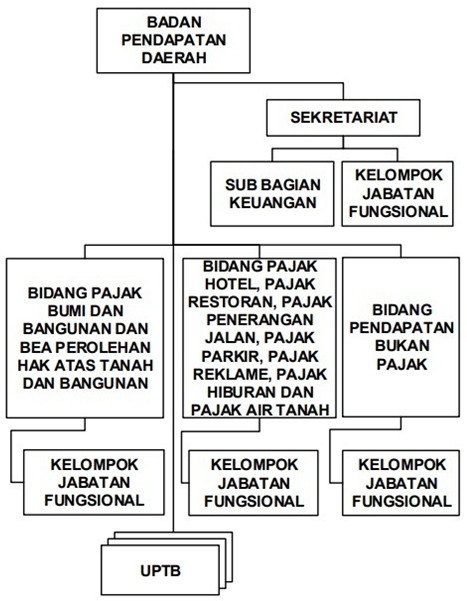
\includegraphics[width=0.54\textwidth]{gambar/struktur-organisasi.png}
    \caption{Struktur Organisasi Bapenda Kota Surabaya}
    \label{fig:struktur-organisasi}
\end{figure}

Berdasarkan struktur organisasi resmi, Badan Pendapatan Daerah (Bapenda) Kota Surabaya dipimpin oleh seorang Kepala Badan. Secara garis besar, struktur ini terbagi menjadi dua komponen utama: unsur pendukung administratif yang direpresentasikan oleh Sekretariat, dan unsur pelaksana teknis yang terdiri dari tiga Bidang utama serta Unit Pelaksana Teknis Badan (UPTB).

Berikut adalah penjelasan rinci mengenai tugas dan fungsi dari setiap unit dalam struktur organisasi Bapenda Kota Surabaya:
\begin{itemize}
    \item Struktur Utama \\
    Struktur utama Bapenda terdiri dari unit-unit yang berfungsi sebagai pendukung jalannya administrasi dan operasional internal organisasi. Unit-unit ini adalah:
    \begin{enumerate}
        \item Badan Pendapatan Daerah: Merupakan unit utama yang memegang tugas pokok untuk mengelola dan mengumpulkan seluruh pendapatan daerah Kota Surabaya.
        \item Sekretariat: Berada langsung di bawah Kepala Badan, Sekretariat memiliki fungsi vital dalam mengurus administrasi umum, kepegawaian, dan mengelola keuangan internal badan.
        \item Sub Bagian Keuangan: Unit ini berada di bawah koordinasi Sekretariat dan memiliki tugas yang lebih spesifik, yaitu secara khusus menangani proses penganggaran serta pembukuan keuangan internal Bapenda.
        \item Kelompok Jabatan Fungsional: Unit ini terdiri dari para pegawai dengan keahlian khusus yang berfungsi untuk mendukung pelaksanaan tugas-tugas teknis organisasi. Seperti yang terlihat pada diagram, Kelompok Jabatan Fungsional ini melekat baik pada Sekretariat maupun pada setiap Bidang Teknis.
    \end{enumerate}
    \item Bidang Teknis dan Pelaksanaan \\
    Bagian ini merupakan unit-unit inti yang melaksanakan fungsi utama Bapenda dalam hal pemungutan pendapatan dari berbagai sektor. Struktur ini terdiri dari tiga bidang utama dan satu unit pelaksana:
    \begin{enumerate}
        \item Bidang PBB dan BPHTB: Bidang ini memiliki fokus teknis untuk mengelola dan memungut pajak yang berkaitan dengan properti dan hak atas tanah. Sesuai dengan yang tertera pada diagram, nama lengkap bidang ini adalah Bidang Pajak Bumi dan Bangunan dan Bea Perolehan Hak atas Tanah.
        \item Bidang Pajak Lainnya: Bidang ini bertanggung jawab mengurus berbagai jenis pajak barang dan jasa di luar PBB dan BPHTB. Rincian tugasnya mencakup pengelolaan Pajak Hotel, Pajak Restoran, Pajak Penerangan Jalan, Pajak Parkir, Pajak Reklame, Pajak Hiburan, dan Pajak Air Tanah.
        \item Bidang Pendapatan Bukan Pajak: Unit teknis ini memiliki tanggung jawab untuk mengelola sumber-sumber pendapatan daerah yang berasal dari luar pajak utama, seperti retribusi daerah dan pendapatan lain-lain di luar pajak.
        \item Unit Pelaksana Teknis Badan (UPTB): Berada di bawah koordinasi dan bertanggung jawab kepada tiga Bidang Teknis, UPTB merupakan unit yang bertugas sebagai pelaksana operasional teknis Bapenda di wilayah-wilayah kerja yang telah ditentukan.
    \end{enumerate}
\end{itemize}
\section{MonPD}
\label{sec:monpd}

MonPD, atau Sistem Monitoring Pendapatan Daerah, adalah sebuah sistem informasi internal yang dimiliki oleh Badan Pendapatan Daerah (Bapenda) Kota Surabaya. Sistem ini dirancang sebagai alat bantu utama bagi pegawai dan pimpinan Bapenda dalam melaksanakan fungsi pengawasan (monitoring) terhadap realisasi penerimaan Pajak Daerah. Fungsi utama dari sistem ini adalah untuk menyajikan data transaksi wajib pajak, memantau setoran pajak, serta menjadi basis data untuk kegiatan pemeriksaan dan penagihan.

Pada kondisi yang ada sekarang (current condition), MonPD versi terdahulu (legacy) dibangun menggunakan teknologi web konvensional yang masih sangat bergantung pada pemrosesan data secara sinkron (synchronous). Dalam operasional hariannya, sistem ini menghadapi kendala teknis yang cukup signifikan, antara lain:

\begin{enumerate}
    \item Arsitektur Data yang Kurang Optimal: \\
    Struktur basis data pada sistem lama belum terorganisir dengan efisien untuk menangani volume data transaksi pajak yang terus bertambah besar.
    \item Mekanisme Pemuatan Data (Data Loading): \\
    Sistem menerapkan pendekatan load data yang tidak efisien, di mana seluruh dataset (ribuan baris data) dimuat secara serentak pada saat halaman pertama kali dibuka. Hal ini menyebabkan beban server menjadi berat dan transfer data (payload) menjadi sangat besar.
    \item Isu Performa: \\
    Akibat dari mekanisme tersebut, waktu tunggu (loading time) untuk membuka satu halaman rekapitulasi bisa mencapai ±120 detik. Kelambatan ini sering kali menghambat produktivitas pegawai dalam melakukan analisis cepat dan pengambilan keputusan di lapangan.
\end{enumerate}

Meskipun secara fungsional sistem ini mampu menampilkan data, namun kendala performa tersebut menuntut adanya peremajaan teknologi yang mendesak agar dapat mengimbangi kebutuhan Bapenda akan data yang real-time dan responsif.
\section{MonPD Reborn}
\label{sec:monpd-reborn}

MonPD Reborn adalah inisiatif pengembangan ulang (redevelopment) dari sistem MonPD terdahulu, yang bertujuan untuk memodernisasi arsitektur sistem dan mengatasi seluruh kendala performa yang ada. Proyek ini bukan sekadar pembaruan tampilan, melainkan pembangunan ulang inti aplikasi menggunakan teknologi terkini berbasis .NET dengan framework ASP.NET Core MVC.

MonPD Reborn dirancang dengan fokus utama pada efisiensi performa dan pengalaman pengguna (User Experience). Perbedaan mendasar dan pembaharuan utama yang ditawarkan oleh MonPD Reborn dibandingkan pendahulunya meliputi:

\begin{enumerate}
    \item Penerapan Teknologi Asinkron (AJAX): \\
    Sistem baru ini mengubah paradigma pemuatan data dari sinkron menjadi asinkron. Aplikasi hanya memuat kerangka halaman terlebih dahulu, kemudian data diambil secara terpisah di latar belakang sesuai permintaan pengguna. Hal ini membuat aplikasi terasa jauh lebih responsif dan ringan.
    \item Antarmuka Interaktif (DevExtreme): \\
    MonPD Reborn mengimplementasikan komponen antarmuka modern yang memungkinkan pengguna melakukan interaksi data tingkat lanjut secara langsung, seperti pemfilteran per kolom, pengurutan data (sorting), dan navigasi halaman (paging) di sisi server, tanpa perlu memuat ulang halaman.
    \item Fitur Visualisasi Data: \\ 
    Sistem ini dilengkapi dengan dashboard analitik yang menyajikan data dalam bentuk grafik, card KPI (Key Performance Indicator), dan pemetaan geospasial (peta sebaran objek pajak) untuk memudahkan pegawai dalam membaca tren pendapatan daerah.
    \item Modul Komprehensif: \\
    MonPD Reborn mengintegrasikan berbagai modul pengawasan yang mencakup Monitoring Objek Pajak, Pengawasan Reklame, Aktivitas Penagihan Wajib Pajak, hingga Laporan Strategis dalam satu platform terpadu.
\end{enumerate}

Melalui pengembangan MonPD Reborn, Bapenda Kota Surabaya menargetkan terciptanya ekosistem kerja digital yang lebih cepat, akurat, dan efisien dalam rangka optimalisasi Pendapatan Asli Daerah (PAD). 
  \cleardoublepage

  % Bab 3 
  \chapter{TINJAUAN PUSTAKA}
\label{chap:tinjauanpustaka}

% Ubah bagian-bagian berikut dengan isi dari tinjauan pustaka
\section{Sistem Informasi Manajemen (SIM)}
\label{sec:sim}

Sistem Informasi Manajemen adalah serangkaian komponen yang saling terkait yang bertujuan untuk mengumpulkan, memproses, menyimpan, dan mendistribusikan informasi untuk mendukung pengambilan keputusan, koordinasi, dan pengendalian dalam suatu organisasi \cite{armah2024sim}. Sistem Informasi Manajemen memiliki tujuan utama untuk mendukung kegiatan operasional dan strategi organisasi dengan cara memberikan informasi yang tepat dan akurat kepada manajemen. Dengan demikian, SIM dapat membantu manajemen dalam mengambil keputusan yang lebih baik, meningkatkan efisiensi dan efektivitas operasional, serta meningkatkan kualitas pengelolaan administrasi. 

Sistem Informasi Manajemen terdiri atas beberapa komponen yang meliputi komponen input, komponen model, komponen output, komponen teknologi, komponen hardware, komponen software, komponen basis data, dan komponen kontrol \cite{rusdiana2014sim}. Seluruh komponen tersebut saling berinteraksi satu sama lain untuk mencapai tujuan sistem informasi manajemen. Penjelasan setiap komponen nya adalah sebagai berikut:

\begin{itemize}
    \item Komponen Input \\
    Input mewakili data yang masuk ke dalam sistem informasi. Input termasuk metode dan media untuk menangkap data yang akan dimasukkan, yang dapat berupa dokumen-dokumen dasar.
    \item Komponen Model \\
    Komponen ini terdiri atas kombinasi prosedur, logika, dan model matematik yang akan memanipulasi data input dan data yang tersimpan di basis data dengan cara yang telah ditentukan untuk menghasilkan keluaran yang diinginkan.
    \item Komponen Output \\
    Hasil dari sistem informasi adalah keluaran informasi yang berkualitas dan dokumentasi yang berguna untuk semua pemakai sistem.
    \item Komponen Teknologi \\
    Teknologi merupakan "tool box" dalam sistem informasi. Teknologi digunakan untuk menerima input, menjalankan model, menyimpan dan mengakses data, menghasilkan dan mengirimkan keluaran, dan membantu pengendalian dari sistem secara keseluruhan.
    \item Komponen Hardware \\
    Hardware berperan penting sebagai suatu media penyimpanan vital bagi sistem informasi yang berfungsi sebagai database sumber data dan informasi untuk memperlancar dan mempermudah kerja dari sistem informasi.
    \item Komponen Software \\
    Software berfungsi sebagai tempat untuk mengolah, menghitung, dan memanipulasi data yang diambil dari hardware untuk menciptakan suatu informasi.
    \item Komponen Basis Data \\
    Basis data (database) merupakan kumpulan data yang saling berkaitan dan berhubungan satu dengan yang lain, tersimpan di perangkat keras komputer dan menggunakan perangkat lunak untuk Sistem Informasi Manajemen memanipulasinya. Data perlu disimpan dalam basis data untuk keperluan penyediaan informasi lebih lanjut. Data dalam basis data perlu diorganisasikan sedemikian rupa informasi yang dihasilkan berkualitas. Organisasi basis data yang baik juga berguna untuk efisiensi kapasitas penyimpanannya. Basis data diakses atau dimanipulasi menggunakan perangkat lunak yang disebut Database Management System (DBMS).
    \item Komponen Kontrol \\
    Banyak hal yang dapat merusak sistem informasi, seperti bencana alam, kegagalan sistem, ketidakefisienan, sabotase, dan sebagainya. Beberapa pengendalian perlu dirancang dan diterapkan untuk meyakinkan bahwa hal yang dapat merusak sistem dapat dicegah ataupun jika telanjur terjadi kesalahan-kesalahan dapat langsung cepat diatasi.
\end{itemize}

Dalam konteks proyek ini, aplikasi Monitoring Pajak Daerah (MonPD Reborn) dikembangkan sebagai wujud dari Sistem Informasi Manajemen. Aplikasi ini berfungsi untuk mengolah data-data transaksi dan realisasi pajak daerah yang bersifat mentah menjadi informasi strategis. Informasi tersebut disajikan dalam bentuk dashboard, rekapitulasi, dan laporan yang membantu pimpinan dan staf di Bapenda Kota Surabaya dalam memantau kinerja penerimaan pajak, mengidentifikasi potensi tunggakan, dan membuat keputusan yang lebih baik terkait strategi optimalisasi pendapatan daerah.
\section{\emph{E-Government}}
\label{sec:e-government}

\emph{Governance} merupakan proses lembaga-lembaga publik dalam mengatasi masalah-masalah publik, mengelola sumber daya publik, dan menjamin realisasi hak asasi manusia secara inklusif. Secara umum \emph{E-Government} dapat dikatakan sebagai suatu aplikasi berbasis komputer dan internet yang digunakan untuk meningkatkan hubungan dan layanan pemerintah kepada warga masyarakatnya. \emph{E-Government} memanfaatan teknologi informasi untuk meningkatkan hubungan dengan pihak-pihak dalam aspek \emph{good governance} (masyarakat dan lembaga bisnis) dengan tujuan meningkatkan kualitas pelayanan yang efektif dan efisien \cite{muliawaty2020egov}.

Proyek MonPD Reborn merupakan bagian dari inisiatif penerapan \emph{E-Government} di lingkungan Pemerintah Kota Surabaya, khususnya pada kategori G2G (\emph{Government-to-Government}). Aplikasi ini tidak berinteraksi langsung dengan masyarakat, melainkan menjadi alat kerja internal bagi para pegawai Bapenda. Dengan menyediakan platform terpusat untuk \emph{monitoring} data pajak, MonPD Reborn mendukung terciptanya pemerintahan yang lebih efisien, responsif, dan akuntabel, sejalan dengan visi Surabaya sebagai \emph{Smart City}.

\section{Pendapatan Asli Daerah (PAD)}
\label{sec:pad}

PAD merupakan akumulasi dari pos penerimaan pajak yang terdiri atas pajak daerah dan retribusi daerah, pos penerimaan non pajak berupa penerimaan hasil perusahaan milik daerah, serta pos penerimaan investasi serta pengelolaan sumber daya alam \cite{nasir2019pad}. PAD bertujuan memberikan kewenangan kepada Pemerintah Daerah untuk mendanai pelaksanaan otonomi daerah sesuai dengan potensi daerah sebagai wujud desentralisasi. Semakin besar dana PAD yang diperoleh oleh daerah akan sebanding dengan laju pembangunan di daerah tersebut. 

Sesuai dengan Undang-Undang No. 33 tahun 2004 tentang perimbangan keuangan antara pusat dan daerah pasal 6 bahwa sumber Pendapatan Asli Daerah meliputi : pajak daerah, retribusi daerah, hasil pengelolaan kekayaan daerah yang dipisahkan, dan lain-lain PAD yang sah. Pendapatan daerah lainnya yang sah yang disebutkan sebelumnya berasal dari hasil penjualan kekayaan daerah yang tidak dipisahkan, jasa giro, pendapatan bunga, keuntungan selisih nilai tukar rupiah terhadap mata uang asing, dan komisi, potongan, ataupun bentuk lain sebagai akibat dari penjualan dan/atau pengadaan barang dan/atau jasa oleh Daerah \cite{uu33_2004}. 

Pajak yang dipungut oleh pemerintah kabupaten/kota berdasarkan Undang-undang (UU) Nomor 1 Tahun 2022 tentang Hubungan Keuangan antara Pemerintah Pusat dan Pemerintah Daerah terdiri atas:

\begin{enumerate}
    \item PBB-P2 (Pajak Bumi dan Bangunan Perdesaan dan Perkotaan)\\
    Contoh: Pajak tahunan yang dibayarkan atas kepemilikan rumah, apartemen, atau ruko di kota tersebut.
    \item BPHTB (Bea Perolehan Hak atas Tanah dan Bangunan)\\
    Contoh: Biaya pajak yang dibayarkan satu kali pada saat membeli rumah baru atau bekas dan melakukan proses balik nama sertifikat.
    \item PBJT (Pajak Barang dan Jasa Tertentu)\\
    Ini adalah gabungan dari beberapa pajak, contoh paling umum adalah:
    \begin{itemize}
        \item Pajak Restoran: Pajak 1\% yang tercantum di struk saat makan di restoran atau kafe.
        \item Pajak Hotel: Pajak yang dibebankan pada tagihan saat menginap di hotel.
        \item Pajak Parkir: Pajak yang pengelola parkir bayarkan (dan biasanya dibebankan ke pengunjung) saat parkir di mal atau gedung perkantoran.
        \item Pajak Hiburan: Pajak pada tiket saat menonton bioskop atau konser.
    \end{itemize}
    \item Pajak Reklame\\
    Contoh: Pajak yang dibayar oleh sebuah toko atau perusahaan untuk memasang papan nama toko, billboard, atau neon box di pinggir jalan.
    \item PAT (Pajak Air Tanah)\\
    Contoh: Pajak yang dibayar oleh pabrik, hotel, atau mal yang menggunakan pompa air sumur bor (air tanah) untuk kegiatan operasionalnya, bukan menggunakan air PDAM.
    \item Pajak MBLB (Pajak Mineral Bukan Logam dan Batuan)\\
    Contoh: Pajak yang dibayar oleh perusahaan tambang pasir, kerikil, atau batu kapur saat mereka mengambil material tersebut dari alam.
    \item Pajak Sarang Burung Walet\\
    Contoh: Pajak yang dibayar oleh seorang pengusaha yang memanen dan menjual sarang burung walet dari gedung atau gua.
    \item Opsen PKB (Opsen Pajak Kendaraan Bermotor)\\
    Contoh: Tambahan biaya (pungutan ekstra) yang nanti akan dikenakan di atas pajak STNK tahunan yang dibayarkan untuk mobil atau motor.
    \item Opsen BBNKB (Bea Balik Nama Kendaraan Bermotor) \cite{uu1_2022}.
    Contoh: Tambahan biaya (pungutan ekstra) yang akan dikenakan di atas biaya normal saat membeli kendaraan baru atau melakukan balik nama kendaraan bekas.
\end{enumerate}
\section{Visual Studio 2022}
\label{sec:vs2022}

Visual Studio 2022 adalah sebuah \emph{Integrated Development Environment} (IDE) atau lingkungan pengembangan terintegrasi yang dikembangkan oleh Microsoft. Sebagai sebuah IDE, Visual Studio 2022 menyediakan rangkaian fasilitas yang komprehensif untuk pengembang perangkat lunak, mulai dari \emph{editor} kode, \emph{compiler}, \emph{debugger}, hingga perancang antarmuka grafis dalam satu aplikasi. Platform ini dirancang untuk meningkatkan produktivitas pengembang dalam membangun berbagai jenis aplikasi, termasuk aplikasi \emph{desktop}, \emph{website}, \emph{mobile}, dan layanan \emph{cloud} \cite{microsoft_vs2022}.

Salah satu pembaruan paling signifikan pada Visual Studio 2022 adalah transisinya menjadi aplikasi 64-bit. Perubahan arsitektur ini memungkinkan Visual Studio untuk mengakses memori yang jauh lebih besar, sehingga mampu membuka, mengedit, dan men-\emph{debug} proyek-proyek berskala besar dan sangat kompleks tanpa mengalami kendala kehabisan memori. Hal ini memberikan peningkatan performa yang drastis, terutama pada saat bekerja dengan solusi yang memiliki ribuan file \cite{microsoft_vs2022_whatsnew}.

Dalam konteks pengembangan aplikasi web dengan ASP.NET, Visual Studio 2022 membawa sejumlah fitur unggulan yang sangat relevan. Fitur \emph{Hot Reload} untuk ASP.NET Core memungkinkan pengembang untuk melihat perubahan pada kode, misalnya pada file C\# atau CSS, secara langsung di aplikasi yang sedang berjalan tanpa perlu menghentikan dan menjalankan ulang proses \emph{debug}. Selain itu, terdapat penyempurnaan pada \emph{editor} Razor dan Blazor, yang mencakup pewarnaan sintaksis yang lebih baik, penyelesaian kode yang lebih cerdas, dan pemformatan otomatis yang lebih rapi \cite{microsoft_vs2022_whatsnew}.

Fitur \emph{Advanced Debugging} memfasilitasi penulis dalam melacak alur data asinkron yang kompleks antara \emph{Controller} dan \emph{ViewModel}, serta memastikan validitas respons data dari server sebelum dirender ke sisi \emph{client}. Fitur-fitur lain seperti \emph{refactoring} cerdas untuk mengganti nama variabel secara aman dan \emph{Quick Actions} untuk memperbaiki masalah kode dengan cepat, semakin memperkuat posisi Visual Studio 2022 sebagai IDE yang andal dan efisien untuk pengembangan proyek ini.

\begin{figure}[ht!]
    \centering
    
\includegraphics[width=0.4\textwidth]{gambar/vs2022.png}
    \caption{Logo Visual Studio 2022}
    \label{fig:vs2022}
\end{figure}

\section{ASP .NET}
\label{sec:aspnet}

ASP.NET adalah salah satu teknologi terbaru di dunia web yang memungkinkan sebuah halaman web bersifat dinamis dan menciptakan komunikasi dua arah (twoway communication) antara client dan server \cite{constantianus2015simta}. ASP.NET merupakan hasil pengembangan lebih dalam dari ASP (Active Server Page) oleh Microsoft. ASP.NET dikembangkan oleh Microsoft yang di-release pertama kali pada Januari 2002 dan berlisensi open source. Framework ini dibangun menggunakan CLR (Common Language Runtime) dan dapat menulis code untuk ASP.NET menggunakan bahasa pemrograman berbasis .NET seperti C\# dan Visual Basic \cite{juyuspan2017aspnetmvc}.

Framework yang dikembangkan oleh Microsoft ini mengimplementasikan arsitektur MVC (Model-View-Controller) dalam membangun aplikasi \cite{christanto2020aspnet}. Arsitektur MVC memisahkan pengembangan aplikasi menjadi tiga komponen utama yang saling berhubungan:

\begin{itemize}
    \item Model: Bagian ini merepresentasikan data dan logika bisnis aplikasi. Model bertanggung jawab penuh atas aturan, validasi, dan manipulasi data. Ia tidak memiliki pengetahuan langsung tentang bagaimana data akan ditampilkan.
    \item View: Komponen ini bertanggung jawab untuk menampilkan data kepada pengguna. View menerima data dari Controller dan menampilkannya dalam format antarmuka (UI) yang sesuai. Pada dasarnya, View adalah templat HTML yang disisipi dengan data dari Model.
    \item Controller: Berperan sebagai jembatan antara Model dan View. Controller menerima input dari pengguna (misalnya, klik tombol atau permintaan URL), berkomunikasi dengan Model untuk memproses permintaan tersebut, lalu memilih View mana yang akan ditampilkan kembali kepada pengguna.
\end{itemize}

Penerapan pola MVC membuat kode program menjadi lebih terstruktur, modular, dan mudah untuk diuji serta dipelihara, yang sangat cocok untuk proyek berskala besar seperti MonPD Reborn.

\begin{figure}[ht!]
    \centering
    
\includegraphics[width=0.4\textwidth]{gambar/asp-net.png}
    \caption{Logo ASP .NET}
    \label{fig:asp-net}
\end{figure}
\section{Visualisasi Data}
\label{sec:visualisasidata}

Visualisasi data merupakan representasi grafis dari data untuk membantu orang memahami konteks dan signifikansi. Tujuan visualisasi data sendiri yakni untuk menyampaikan informasi secara ringkas dan jelas sehingga mudah dipahami oleh pembaca \cite{alghivary2023visualisasi}. Dengan menggunakan elemen visual seperti bagan, grafik, dan peta, visualisasi data menyediakan cara yang mudah diakses untuk melihat dan memahami tren, pencilan (outliers), dan pola dalam data. Dalam lingkungan organisasi, visualisasi data memungkinkan para pengambil keputusan untuk melihat analitik yang disajikan secara visual, sehingga mereka dapat memahami konsep yang sulit atau mengidentifikasi pola baru.

Prinsip visualisasi data diterapkan secara langsung pada User Interface (UI) website MonPD Reborn. Seluruh halaman pada website ini menggunakan berbagai komponen visual seperti card, tabel, grafik, dan lainnya untuk menampilkan data statistik, diagram batang untuk perbandingan, dan tabel data berwarna untuk status. Tujuan utamanya adalah agar pengguna dapat dengan cepat memahami kondisi terkini dari realisasi dan pemeriksaan pajak tanpa harus membaca laporan tekstual yang panjang dan kompleks.

\section{\emph{Entity Framework Core} (EF Core)}
\label{sec:efcore}

Entity Framework Core (EF Core) adalah kerangka kerja \emph{Object-Relational Mapper} (ORM) yang direkomendasikan untuk .NET, yang sebelumnya dikenal sebagai .NET Core. Sebagai penerus EF6, EF Core telah sepenuhnya direkayasa ulang dan dijadikan \emph{open source} di GitHub. EF Core dikembangkan oleh Microsoft sehingga memungkinkan pengguna untuk memetakan kelas-kelas C\# ke tabel-tabel \emph{database}. Ini memungkinkan pengguna berinteraksi dengan \emph{database} menggunakan kode C\# alih-alih menulis \emph{query} SQL secara langsung \cite{patel_medium_efcore}. Fitur-fitur utama dari EF Core diantaranya:

\begin{itemize}
    \item \emph{Cross-Platform Support}: Dapat digunakan di Windows, macOS, dan Linux.
    \item LINQ \emph{Support}: Memungkinkan Anda menggunakan LINQ (\emph{Language Integrated Query}) untuk melakukan kueri \emph{database}.
    \item Pelacakan Perubahan: Secara otomatis melacak perubahan dalam data, sehingga memudahkan untuk memperbarui catatan.
    \item Migrasi: Memungkinkan Anda untuk mengelola dan menerapkan perubahan skema pada \emph{database} dari waktu ke waktu.
\end{itemize}

EF Core menggunakan \texttt{DbContext}, yang merepresentasikan sesi dengan \emph{database} dan memungkinkan pengguna untuk melakukan \emph{query} dan menyimpan data. Kelas C\# yang juga dikenal sebagai \emph{entity}, dipetakan ke tabel \emph{database}, dan properti kelas tersebut dipetakan ke kolom dalam tabel. Alur ini dapat dibagi menjadi tiga konsep utama:

\begin{itemize}
    \item \emph{Model}: Kelas-kelas C\# merepresentasikan struktur \emph{database}.
    \item \emph{Context}: Kelas \texttt{DbContext} yang menangani operasi \emph{database} seperti \emph{query}, menambah, memperbarui, dan menghapus data.
    \item \emph{Database Provider}: EF Core mendukung berbagai \emph{database} seperti SQL Server, MySQL, PostgreSQL, dan SQLite melalui penyedia \emph{database}.
\end{itemize}

Dengan menggunakan EF Core, pengembang dapat lebih fokus pada logika bisnis aplikasi tanpa harus terlalu khawatir tentang detail implementasi \emph{database}, sehingga mempercepat proses pengembangan aplikasi. EF Core berperan sebagai jembatan komunikasi otomatis antara logika aplikasi MonPD Reborn dengan \emph{database} Oracle di Bapenda tanpa perlu menulis kueri SQL manual yang kompleks.

\begin{figure}[ht!]
    \centering
    
\includegraphics[width=0.4\textwidth]{gambar/logo/efcore.png}
    \caption[Logo EF Core]{Logo EF Core \cite{logo_efcore}}
    \label{fig:efcore}
\end{figure}
\section{Oracle}
\label{sec:oracle}

Oracle adalah perusahaan teknologi informasi yang berbasis di AS yang menyediakan berbagai produk dan layanan bisnis, termasuk Oracle Database, sistem manajemen basis data relasional (RDBMS) \cite{ibm_oracle_2024}. Oracle Database adalah produk unggulan Oracle yang merupakan sistem manajemen basis data dan pergudangan populer yang digunakan oleh organisasi di seluruh dunia untuk mengelola dan menyimpan data mereka. Basis data ini menggunakan SQL untuk manipulasi dan query dan merupakan basis data pertama dari jenisnya yang ditawarkan untuk rilis komersial. Oracle Database dapat dijalankan di Linux atau Microsoft Windows. Oracle dikenal luas karena keandalannya (robustness), skalabilitasnya yang tinggi, fitur keamanannya yang komprehensif, dan kemampuannya untuk menangani beban kerja yang sangat besar dan kompleks.

Penerapan Oracle Database sebagai fondasi untuk sistem krusial seperti Monitoring Pajak Daerah (MonPD Reborn) memberikan landasan teknologi yang sangat kuat dan dapat diandalkan, jauh melampaui sekadar penyimpanan data. Keunggulan utamanya terletak pada keandalan transaksional yang dijamin oleh properti ACID (Atomicity, Consistency, Isolation, Durability), yang memastikan setiap data realisasi, pemeriksaan, atau pelanggaran pajak tercatat secara akurat, konsisten, dan tanpa anomali. Selain itu, dari sisi kinerja dan ketersediaan tinggi, arsitektur Oracle dirancang untuk menangani ribuan transaksi simultan dengan waktu respons yang cepat, sehingga aplikasi MonPD Reborn tetap responsif bahkan saat diakses oleh banyak pengguna atau saat menjalankan query laporan yang kompleks. Kemampuan ini disempurnakan lebih lanjut oleh PL/SQL, yang memungkinkan logika bisnis dan validasi aturan perpajakan yang rumit untuk diimplementasikan langsung di dalam database sebagai stored procedures dan triggers. Dengan demikian, konsistensi aturan terjaga di seluruh aplikasi dan proses audit menjadi lebih mudah. 

Secara keseluruhan, kombinasi antara integritas data, keamanan, skalabilitas, dan kemampuan pemrosesan logika terpusat menjadikan Oracle Database pilihan ideal yang memastikan aplikasi MonPD Reborn tidak hanya fungsional, tetapi juga aman, auditable, dan memiliki performa tinggi sesuai dengan standar tata kelola pemerintahan yang baik.

\begin{figure}[ht!]
    \centering
    
\includegraphics[width=0.4\textwidth]{gambar/oracle.png}
    \caption{Logo Oracle}
    \label{fig:oracle}
\end{figure}
\section{DevExtreme}
\label{sec:devextreme}

DevExtreme adalah sebuah \emph{suite} komponen \emph{User Interface} (UI) komprehensif yang dikembangkan oleh DevExpress \cite{devexpress_js_dev}. Rangkaian \emph{tool} ini dirancang untuk membantu pengembang membangun aplikasi web yang kaya fitur, responsif, dan memiliki kinerja tinggi dengan lebih cepat. Dibuat menggunakan HTML5, JavaScript, dan CSS. DevExtreme menawarkan koleksi \emph{widget} yang luas, mulai dari \emph{data grid} yang kompleks, \emph{chart} interaktif, hingga \emph{editor} data dan elemen navigasi. Keunggulan utamanya terletak pada fleksibilitasnya, di mana komponen-komponen ini dapat diintegrasikan dengan mudah ke dalam berbagai arsitektur aplikasi dan \emph{framework} populer, termasuk ASP.NET Core, Angular, React, dan Vue, memungkinkan pengembangan antarmuka yang modern dan konsisten di berbagai platform.

Dalam konteks pengembangan proyek Monitoring Pajak Daerah (MonPD Reborn), \emph{library} DevExtreme, khususnya komponen DataGrid for ASP.NET Core, memegang peranan krusial. Komponen ini dimanfaatkan untuk menampilkan data rekapitulasi pajak yang kompleks dalam format tabel yang terstruktur dan mudah dianalisis. Fitur-fitur spesifik seperti kolom bertingkat (\emph{banded columns}) digunakan untuk mengelompokkan data secara logis (misalnya, mengelompokkan kolom di bawah kategori "Realisasi" dan "Pemeriksaan"). Selain itu, fungsionalitas bawaan seperti kalkulasi ringkasan (\emph{summary}), pemfilteran (\emph{filtering}), dan pengurutan data (\emph{sorting}) diimplementasikan untuk memberikan pengalaman interaktif kepada pengguna. Penggunaan komponen DataGrid dari DevExtreme secara signifikan mempercepat proses pengembangan, karena menyediakan fungsionalitas canggih yang siap pakai, sehingga pengembang dapat lebih fokus pada implementasi logika bisnis di sisi \emph{back-end}.

\section{JQuery}
\label{sec:jquery}

jQuery adalah sebuah library JavaScript yang cepat, ringan, dan kaya fitur. Ini adalah library yang paling banyak digunakan dalam sejarah pengembangan web, meskipun popularitasnya kini bersaing dengan framework modern. Misi utama jQuery diciptakan adalah untuk menyederhanakan skrip di sisi klien (client-side scripting), yang terangkum dalam motonya: "Write Less, Do More" \cite{jquery_official}.

Pada dasarnya, jQuery membungkus fungsi-fungsi JavaScript yang umum namun kompleks, seperti manipulasi Document Object Model (DOM), penanganan event, dan panggilan AJAX, ke dalam method yang jauh lebih sederhana dan mudah digunakan. Fungsionalitas utamanya mencakup:

\begin{enumerate}
    \item Manipulasi DOM: Mempermudah proses pemilihan elemen HTML (menggunakan sintaks selektor CSS) serta mengubah atribut, style, dan kontennya.
    \item Penanganan Event (Event Handling): Menyediakan cara yang ringkas dan konsisten antar browser untuk merespons interaksi pengguna, seperti .click(), .hover(), atau .change().
    \item Panggilan AJAX: Menyediakan method yang kuat dan mudah seperti \$.ajax(), .get(), dan .post() yang secara drastis menyederhanakan proses pengiriman dan penerimaan data dari server.
\end{enumerate}

Dalam konteks proyek MonPD Reborn, library jQuery memegang peranan vital sebagai alat untuk menangani semua interaksi pengguna dan sebagai fondasi untuk mengimplementasikan teknik pemuatan data asinkron melalui fungsi \$.ajax().
\section{\emph{Asynchronous JavaScript and XML} (AJAX)}
\label{sec:ajax}

AJAX bukanlah sebuah bahasa pemrograman, melainkan sebuah teknik atau pendekatan pengembangan web untuk menciptakan aplikasi yang cepat dan dinamis \cite{aws_ajax}. AJAX merupakan singkatan dari \emph{Asynchronous JavaScript and XML}. Teknik ini memungkinkan halaman web untuk berkomunikasi dengan \emph{server} di latar belakang (mengirim dan mengambil data) secara asinkron tanpa harus memuat ulang (\emph{refresh}) seluruh halaman \cite{w3schools_ajax}.

Konsep "asinkron" adalah kuncinya. Konsep ini berarti bahwa \emph{browser} tidak "dibekukan" dan dapat terus merespons interaksi pengguna (seperti \emph{scrolling} atau input lain) sementara permintaan data ke \emph{server} sedang diproses di latar belakang. Saat data diterima dari \emph{server} (yang kini lebih umum menggunakan format JSON daripada XML), JavaScript akan mengambil alih untuk memperbarui bagian spesifik dari halaman (DOM) dengan data baru tersebut.

Inti dari teknologi AJAX di dalam \emph{browser} adalah objek \emph{XMLHttpRequest} (XHR). Objek inilah yang bertugas membuka koneksi, mengirim permintaan, dan menerima respons dari \emph{server}. \emph{Library} seperti jQuery kemudian membungkus penggunaan objek XHR yang kompleks ini ke dalam fungsi yang sederhana seperti \texttt{\$.ajax()}.

Pada proyek MonPD Reborn, teknik AJAX adalah solusi fundamental untuk mengatasi masalah performa. Daripada memuat seluruh data secara serentak saat halaman dibuka, aplikasi menggunakan panggilan AJAX untuk memuat data \emph{Partial View} (seperti tabel dan detail) hanya pada saat data tersebut dibutuhkan oleh pengguna. 


  \cleardoublepage

  % Bab 4 
  \chapter{PEMBAHASAN}
\label{chap:pembahasan}

% Ubah bagian-bagian berikut dengan isi dari pendahuluan
\section{Tinjauan Kasus}
\label{sec:tinjauankasus}

Proyek yang dikerjakan selama periode magang di Badan Pendapatan Daerah (Bapenda) Kota Surabaya adalah "Pengembangan Sistem Monitoring Pendapatan Daerah (MonPD Reborn) Berbasis .NET". Proyek ini berfokus pada perancangan dan implementasi beberapa modul vital dalam sebuah sistem informasi internal yang bertujuan untuk meningkatkan efektivitas pengawasan, penagihan, dan analisis data perpajakan daerah.

Sistem ini dirancang untuk dapat diakses oleh pegawai internal Bapenda dengan tujuan utama menyediakan dashboard analitik dan tabel data yang interaktif. Website ini dibangun untuk mengolah dan memvisualisasikan data dari berbagai jenis pajak, seperti Pajak Reklame, Hotel, Restoran, dan lainnya. Tujuannya adalah untuk memberikan pandangan yang komprehensif dan real-time mengenai aktivitas wajib pajak (WP), realisasi target pendapatan, serta progres aktivitas lapangan seperti pemeriksaan dan penagihan, sehingga dapat mendukung pengambilan keputusan yang lebih cepat dan berbasis data.

\section{Analisis dan Perancangan Sistem}
\label{sec:analisisperancangansistem}

Analisis sistem dilakukan untuk memahami alur kerja internal Bapenda serta kebutuhan fungsional dari setiap modul yang akan dikembangkan. Hasil analisis ini kemudian menjadi dasar dalam perancangan arsitektur sistem, struktur \emph{ViewModel}, dan desain antarmuka pengguna.

\subsection{Analisis Kebutuhan Fungsional}
Berdasarkan diskusi dan analisis, diidentifikasi kebutuhan fungsional yang menjadi dasar pengembangan MonPD Reborn. Detailnya disajikan dalam Tabel \ref{tab:kebutuhan_fungsional}.

\renewcommand{\arraystretch}{1.5}

% Menggunakan kolom p{} agar teks membungkus (wrap) dengan benar di kertas A5
\begin{longtable}{|c|p{2cm}|p{2cm}|p{4cm}|}
\caption{Analisis Kebutuhan Fungsional MonPD Reborn}
\label{tab:kebutuhan_fungsional} \\
\hline
\textbf{No} & \textbf{Menu Utama} & \textbf{Sub-menu} & \textbf{Deskripsi Kebutuhan} \\ \hline
\endfirsthead

\hline
\textbf{No} & \textbf{Menu Utama} & \textbf{Sub-menu} & \textbf{Deskripsi Kebutuhan} \\ \hline
\endhead

\hline
\endfoot

\hline
\endlastfoot

1 & \multirow{8}{2cm}{Objek Pajak} & Series Pendapatan & Menampilkan data historis pendapatan daerah dalam bentuk \emph{series}. \\ \cline{1-1} \cline{3-4}
2 &  & Pengedokan Pajak & Modul untuk memantau aktivitas pendataan potensi pajak di lapangan. \\ \cline{1-1} \cline{3-4}
3 &  & Pemeriksaan Pajak & Menampilkan rekapitulasi dan detail hasil pemeriksaan objek pajak. \\ \cline{1-1} \cline{3-4}
4 &  & Alat Rekam \emph{Online} & Memonitor data dari alat rekam transaksi (\emph{tapping box}). \\ \cline{1-1} \cline{3-4}
5 &  & Realisasi Kontrol & Menyajikan perbandingan antara target dan realisasi secara detail. \\ \cline{1-1} \cline{3-4}
6 &  & Data OP & Akses untuk melihat dan mengelola data \emph{master} Objek Pajak. \\ \cline{1-1} \cline{3-4}
7 &  & Monitoring Capaian & \emph{Dashboard} untuk memantau progres pencapaian target. \\ \cline{1-1} \cline{3-4}
8 &  & Monitoring Wilayah & Membandingkan capaian pendapatan antar wilayah kerja (UPTB). \\ \hline

9 & \multirow{4}{2cm}{Pengawasan Reklame} & Reklame \emph{Summary} & Menampilkan ringkasan data agregat jumlah reklame dan potensi pendapatan. \\ \cline{1-1} \cline{3-4}
10 &  & Kontrol Reklame & Modul melakukan kontrol dan validasi terhadap data reklame. \\ \cline{1-1} \cline{3-4}
11 &  & Reklame Liar & Mencatat laporan mengenai reklame yang tidak berizin. \\ \cline{1-1} \cline{3-4}
12 &  & Pendataan Reklame & Antarmuka untuk proses pendataan titik reklame baru. \\ \hline

13 & \multirow{4}{2cm}{Wajib Pajak} & Aktivitas Penghimbauan & Mencatat dan memonitor kegiatan penghimbauan kepada WP. \\ \cline{1-1} \cline{3-4}
14 &  & Aktivitas Peneguran & Melacak pengiriman surat teguran kepada WP yang menunggak. \\ \cline{1-1} \cline{3-4}
15 &  & Aktivitas Penagihan & Memantau siklus penagihan aktif. \\ \cline{1-1} \cline{3-4}
16 &  & Data WP & Akses terpusat profil dan riwayat data Wajib Pajak. \\ \hline

17 & \multirow{2}{2cm}{Laporan Strategis} & Evaluasi Target & Laporan perbandingan target dengan realisasi periode tertentu. \\ \cline{1-1} \cline{3-4}
18 &  & Analisis Tren & Menyajikan analisis kenaikan atau penurunan pendapatan. \\ \hline
\end{longtable}


\subsection{Perancangan Arsitektur Sistem}
Sistem ini dibangun menggunakan arsitektur \emph{Model View Controller} (MVC) yang disediakan oleh \emph{framework} ASP.NET Core dengan bahasa pemrograman C\#. Pola arsitektur ini dipilih karena kemampuannya memisahkan antara logika bisnis, data, dan presentasi, sehingga menghasilkan struktur kode yang rapi, modular, dan mudah dikelola.
\begin{itemize}
    \item \textbf{\emph{Model}}: \\
    Terdiri dari serangkaian kelas \emph{ViewModel} (VM) yang dirancang khusus untuk setiap halaman. \emph{ViewModel} ini berfungsi sebagai ``cetakan'' data yang akan dikirim ke antarmuka, menggabungkan data dari berbagai sumber dan mengolahnya sesuai kebutuhan tampilan. Di dalam \emph{ViewModel}, terdapat juga kelas \emph{Method} yang berisi logika untuk mengambil dan memanipulasi data (baik data \emph{dummy} maupun dari basis data). \\
    Salah satu keputusan desain arsitektur yang penting adalah menempatkan sebagian besar logika bisnis di dalam \emph{Method} pada setiap \emph{ViewModel}. Dengan pendekatan ini, \emph{Controller} hanya bertugas sebagai penerus permintaan. Contohnya, pada \emph{ViewModel} \texttt{ReklameLiarVM}, terdapat lebih dari 5 \emph{class} yang berbeda (\texttt{Index}, \texttt{Show}, \texttt{Detail}, \texttt{RekapBulanan}, \texttt{DetailData}) untuk melayani setiap kebutuhan data yang spesifik, mulai dari data rekap bulanan hingga data detail untuk \emph{modal pop-up}.
    \item \textbf{\emph{View}}: \\
    Terdiri dari file-file \texttt{.cshtml} (\emph{Razor}) yang bertanggung jawab untuk menampilkan antarmuka pengguna. Halaman \emph{View} menerima data dari \emph{Controller} melalui objek \emph{ViewModel} dan menampilkannya dalam bentuk \emph{dashboard}, tabel, dan formulir. Sebagian besar tampilan tabel interaktif diimplementasikan menggunakan komponen dari \texttt{DevExtreme}.
    \item \textbf{\emph{Controller}}: \\
    Berperan sebagai jembatan antara \emph{Model} dan \emph{View}. \emph{Controller} menerima permintaan HTTP dari pengguna (misalnya, saat filter diterapkan), memanggil \emph{Method} yang sesuai di dalam \emph{ViewModel} untuk mendapatkan data, lalu mengirimkan data tersebut ke \emph{View} yang relevan untuk ditampilkan kepada pengguna.
\end{itemize}

\subsection{Perancangan \emph{Database}}
Aplikasi ini berinteraksi dengan basis data yang sudah ada di \emph{server database} Bapenda. Koneksi dan manipulasi data dari aplikasi ke basis data ditangani menggunakan \emph{Entity Framework Core}, dengan kelas \texttt{DBContext} yang berfungsi sebagai gerbang utama. Data yang digunakan selama pengembangan bersifat data riil, sehingga struktur \emph{ViewModel} dan logika aplikasi dirancang untuk dapat terhubung langsung dengan tabel-tabel utama seperti \texttt{TPemeriksaan}, \texttt{DbMonResto}, \texttt{DbMonParkir}, dan lainnya, yang merepresentasikan data riil di \emph{server database} Bapenda.

\subsection{Perancangan Antarmuka (UI/UX)}

Perancangan antarmuka pada sistem MonPD Reborn dilakukan dengan mengedepankan prinsip \emph{Information Hierarchy} dan efisiensi operasional. Mengingat sistem ini digunakan untuk memonitor data perpajakan yang sangat besar, setiap halaman dirancang untuk meminimalkan beban kognitif pengguna melalui penempatan elemen yang strategis. Berikut adalah rincian rancangan tata letak dan fungsionalitas pada setiap bagian utama sistem:

\begin{itemize}
    \item Rancangan Pusat Komando (\emph{Command Center}) \\
    Tampilan utama atau \emph{dashboard} dirancang menggunakan tata letak berbasis kartu (\emph{card-based layout}) untuk memberikan ringkasan performa seluruh jenis pajak dalam satu layar tunggal sebagaimana ditunjukkan pada Gambar \ref{fig:wireframe-dashboard-utama-monpd}.
    \begin{figure}[H]
        \centering
        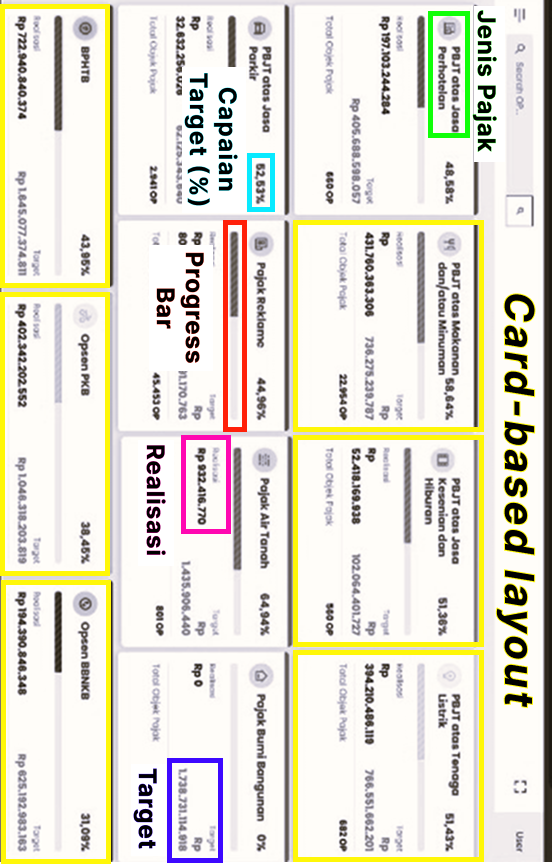
\includegraphics[width=0.9\textwidth]{gambar/wireframe-dashboard-utama-monpd.png}
        \caption{\emph{Wireframe Dashboard} Utama MonPD Reborn}
        \label{fig:wireframe-dashboard-utama-monpd}
    \end{figure}
    \begin{itemize}
        \item \textbf{Fitur Utama:}
            \begin{itemize}
                \item \textbf{Jenis Pajak:} Menampilkan label jenis pajak (eg: Perhotelan, Restoran, Parkir) untuk memudahkan klasifikasi data.
                \item \textbf{Metrik Capaian:} Persentase angka realisasi terhadap target yang dihitung secara \emph{real-time} untuk memberikan indikator kinerja utama.
                \item \textbf{Indikator Visual:} \emph{Progress bar} yang memberikan representasi visual dari persentase capaian memudahkan pemindaian cepat.
                \item \textbf{Komparasi Finansial:} Penyajian nominal Realisasi (pendapatan yang sudah masuk) dan Target (sasaran tahunan).
            \end{itemize}

        \item \textbf{Analisis Penempatan:}
            \begin{itemize}
                \item \textbf{Hierarki Informasi Kartu:} Penggunaan \emph{card-based layout} berfungsi untuk melakukan enkapsulasi data. Setiap jenis pajak memiliki kontainer visualnya sendiri, mencegah terjadinya tumpang tindih informasi antar sektor pajak yang berbeda.
                \item \textbf{Strategi \emph{Visual Cues}:} Penempatan Metrik Capaian dan \emph{Progress Bar} diletakkan di bagian atas kartu. Hal ini didasarkan pada pola baca pengguna yang cenderung memprioritaskan kesimpulan performa (pencapaian) sebelum melihat rincian nominal pendukungnya.
                \item \textbf{Penyandingan Vertikal:} Nominal Realisasi diletakkan di sebelah nominal Target. Penempatan ini dirancang untuk mempermudah perbandingan visual langsung antar dua angka finansial yang berkaitan, sehingga pengguna dapat langsung mengetahui selisih antara pencapaian saat ini dengan target akhir.
            \end{itemize}
    \end{itemize}

    \item Rancangan Struktur Modul Analitik \\
    Setiap modul analitik (misalnya Monitoring Wilayah) menggunakan \emph{standardized template} tiga lapis yang konsisten untuk menciptakan alur kerja yang intuitif bagi pengguna sebagaimana ditunjukkan pada Gambar \ref{fig:wireframe-dashboard-menu-monpd}.
    \begin{figure}[H]
        \centering
        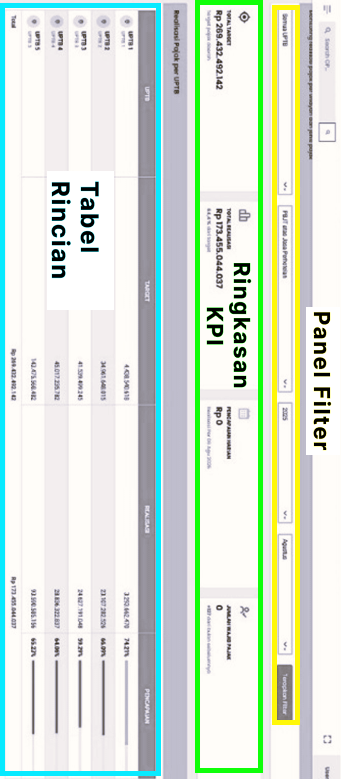
\includegraphics[width=0.65\textwidth]{gambar/wireframe-dashboard-menu-monpd.png}
        \caption{\emph{Wireframe Dashboard} Menu MonPD Reborn}
        \label{fig:wireframe-dashboard-menu-monpd}
    \end{figure}
    \begin{itemize}
        \item \textbf{Fitur Utama:}
            \begin{itemize}
                \item \textbf{Panel Filter:} Terdiri dari komponen \emph{dropdown} untuk pemilihan wilayah (UPTB), jenis pajak, tahun, dan bulan, serta tombol eksekusi "Terapkan Filter".
                \item \textbf{Ringkasan KPI:} Menampilkan kartu-kartu metrik utama (\emph{Key Performance Indicators}) seperti Total Target, Total Realisasi, Pencapaian Harian, dan Jumlah Wajib Pajak (ini bukan standar, karena KPI tiap menu memiliki komponen berbeda).
                \item \textbf{Tabel Rincian:} Menyajikan data rincian per baris yang dilengkapi dengan kolom Target, Realisasi, serta visualisasi \emph{progress bar} untuk setiap baris data.
            \end{itemize}

        \item \textbf{Analisis Penempatan:}
            \begin{itemize}
                \item \textbf{Strategi \emph{Top-Down Workflow}:} Penempatan \textbf{Panel Filter} di posisi teratas berfungsi sebagai gerbang utama operasional. Hal ini menerapkan prinsip \emph{Progressive Disclosure}, di mana sistem membatasi pemuatan data secara masif di awal untuk menjaga performa (\emph{load time}), dan baru akan menarik data spesifik setelah pengguna menentukan parameter pilihannya.
                \item \textbf{Hierarki Kognitif \emph{Summary-to-Detail}:} \textbf{Ringkasan KPI} diletakkan di bagian tengah sebagai jembatan informasi. Secara psikologis, pengguna memerlukan konklusi cepat (angka agregat) segera setelah menerapkan filter, sebelum akhirnya melakukan eksplorasi mendalam pada data baris demi baris di bagian bawah.
                \item \textbf{Optimalisasi Ruang Kerja Tabel:} \textbf{Tabel Rincian} diletakkan sebagai elemen paling luas di bagian bawah. Penempatan ini memberikan ruang visual yang maksimal bagi komponen \emph{DevExtreme DataGrid} untuk menampilkan banyak kolom data secara komprehensif tanpa terasa sesak, sehingga memudahkan proses analisis rincian transaksi oleh pegawai Bapenda.
            \end{itemize}
    \end{itemize}

    \item Rancangan Interaktivitas Data (\emph{DataGrid}) \\
    Komponen \emph{DataGrid} dirancang sebagai pusat eksplorasi data yang memungkinkan pengguna melakukan manipulasi informasi secara mandiri tanpa perlu bergantung pada proses pemuatan ulang halaman (\emph{refresh}) sebagaimana ditunjukkan pada Gambar \ref{fig:wireframe-datagrid}.
    \begin{figure}[H]
        \centering
        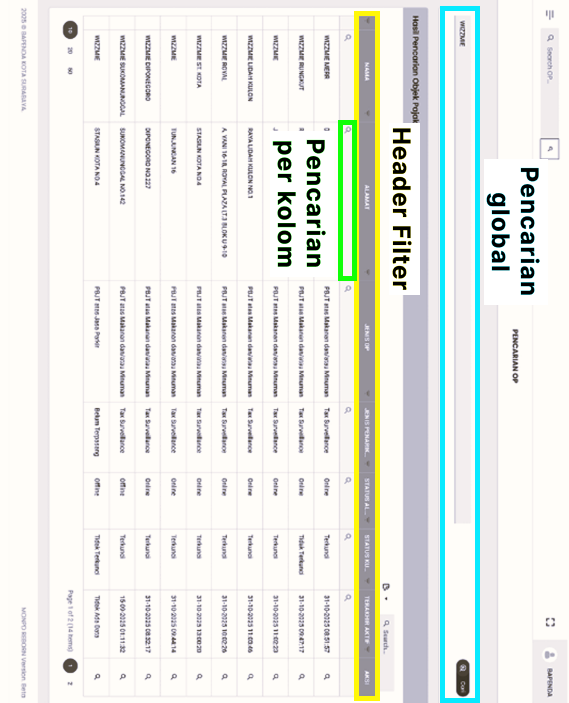
\includegraphics[width=0.96\textwidth]{gambar/wireframe-datagrid.png}
        \caption{\emph{Wireframe DataGrid}}
        \label{fig:wireframe-datagrid}
    \end{figure}
    \begin{itemize}
        \item \textbf{Fitur Utama:}
            \begin{itemize}
                \item \textbf{Pencarian Global:} Fitur pencarian tingkat tinggi di pojok kanan atas yang memungkinkan pengguna mencari kata kunci tertentu di seluruh kolom tabel secara simultan.
                \item \textbf{\emph{Header Filter} dan \emph{Sorting}:} Setiap judul kolom (\emph{Nama, Alamat, Jenis OP}, dll.) dilengkapi dengan fungsi pengurutan (\emph{sorting}) naik atau turun serta filter nilai unik (\emph{header filter}) untuk mempersempit kategori data.
                \item \textbf{Pencarian Per Kolom:} Baris filter (\emph{filter row}) yang terletak tepat di bawah \emph{header}. Fitur ini memungkinkan pengguna melakukan penyaringan data secara spesifik pada kolom tertentu, seperti mencari nama Wajib Pajak tanpa mencampuradukkan dengan data alamat.
                \item \textbf{Navigasi Halaman:} Terletak di bagian bawah kiri, fitur ini membatasi jumlah data yang tampil per layar untuk menjaga performa \emph{rendering} pada sisi \emph{client}.
            \end{itemize}

        \item \textbf{Analisis Penempatan:}
            \begin{itemize}
                \item \textbf{Konvensi Standar Pencarian Global:} Penempatan \textbf{Pencarian Global} di bagian atas kanan mengikuti standar \emph{User Interface} yang umum, memudahkan pengguna baru untuk langsung mengenali titik awal pencarian informasi secara cepat.
                \item \textbf{Kedekatan Kontekstual:} Penempatan \textbf{Pencarian Per Kolom} dan \textbf{\emph{Header Filter}} yang melekat langsung pada baris judul kolom bertujuan untuk efisiensi kognitif. Pengguna tidak perlu memindahkan fokus pandangan terlalu jauh dari data yang sedang diamati untuk melakukan penyaringan informasi yang lebih granular.
                \item \textbf{Kontrol Presisi Data:} Dengan adanya baris filter khusus per kolom, beban kerja sistem menjadi lebih efisien karena kueri yang dikirim ke server (\emph{server-side filtering}) menjadi lebih spesifik, mengurangi potensi beban \emph{payload} data yang tidak relevan.
                \item \textbf{Manajemen Beban Visual:} \textbf{\emph{Pagination}} diletakkan di bagian akhir alur konsumsi data (bawah). Hal ini memastikan pengguna hanya fokus pada subset data tertentu pada satu waktu, yang secara teknis mendukung tujuan utama \emph{MonPD Reborn} dalam mereduksi waktu muat data secara signifikan.
            \end{itemize}
    \end{itemize}

    \item Rancangan \emph{Drill-down} dan \emph{Pop-up} Detail \\
    Untuk memberikan akses informasi yang lebih mendalam tanpa mengganggu alur kerja pengguna, sistem menyediakan fitur \emph{drill-down} yang memungkinkan rincian data tampil secara transisi.    
    \begin{itemize}
        \item \textbf{Fitur:} Jendela \emph{modal pop-up} yang menampilkan rincian transaksi individu secara spesifik.
        \item \textbf{Analisis Penempatan:} Penggunaan jendela \emph{modal} di atas halaman utama bertujuan untuk menjaga \emph{context-awareness} pengguna. Dengan tetap menampilkan latar belakang halaman rekapitulasi yang sedikit meredup, pengguna akan tetap ingat pada parameter filter atau kategori data awal yang sedang mereka amati saat melihat detail transaksi.
    \end{itemize}

    \item Rancangan Visualisasi Geospasial \\
    Penyajian data berbasis lokasi dirancang untuk memberikan pemahaman spasial terhadap sebaran objek pajak di wilayah Kota Surabaya sebagaimana ditunjukkan pada Gambar \ref{fig:wireframe-geospasial}.
    \begin{figure}[H]
        \centering
        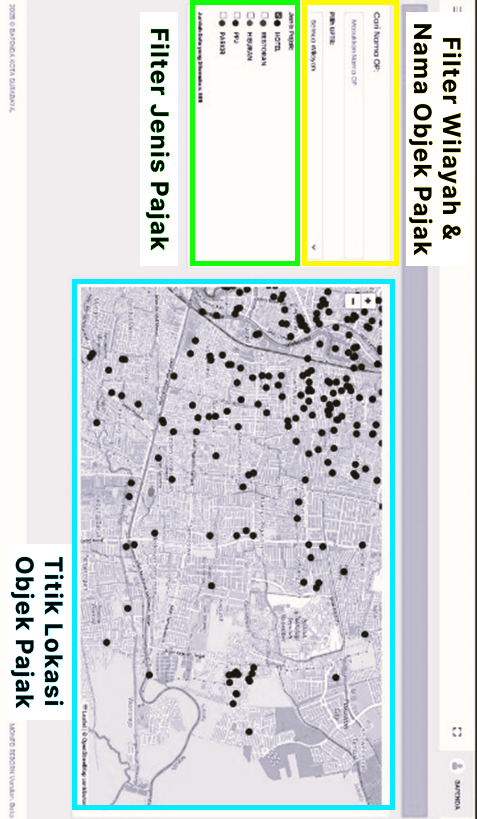
\includegraphics[width=0.73\textwidth]{gambar/wireframe-geospasial.png}
        \caption{Wireframe Visualisasi Geospasial}
        \label{fig:wireframe-geospasial}
    \end{figure}
    \begin{itemize}
        \item \textbf{Fitur Utama:}
            \begin{itemize}
                \item \textbf{Kontrol Pencarian dan Wilayah:} Terdiri dari kolom input "Cari Nama OP" untuk pencarian spesifik entitas pajak dan \emph{dropdown} "Pilih UPTB" untuk membatasi cakupan wilayah kerja administratif.
                \item \textbf{Filter Kategori:} Menyediakan daftar pilihan \emph{checkbox} jenis pajak (Hotel, Restoran, Hiburan, PPJ, Parkir) yang memungkinkan pengguna melakukan \emph{overlaying} data dari berbagai sektor pajak secara bersamaan.
                \item \textbf{Kanvas Pemetaan:} Area peta interaktif yang menampilkan \emph{plotting} titik-titik koordinat objek pajak secara \emph{real-time} berdasarkan parameter filter yang diterapkan.
            \end{itemize}

        \item \textbf{Analisis Penempatan:}
            \begin{itemize}
                \item \textbf{Aksesibilitas Kontrol:} Penempatan panel filter di sisi atas dan samping kiri mengikuti pola pandangan manusia yang memulai pemindaian dari pojok kiri atas. Hal ini memastikan pengguna dapat dengan cepat memodifikasi parameter data sebelum beralih ke analisis visual pada peta.
                \item \textbf{Fokus Analisis Spasial:} Area peta diletakkan sebagai elemen pusat dengan dimensi paling luas. Penempatan ini bertujuan untuk meminimalisir distraksi visual lain, sehingga tim lapangan dapat memfokuskan perhatian sepenuhnya pada kepadatan (\emph{clustering}) titik objek pajak.
                \item \textbf{Efisiensi Perencanaan Rute:} Integrasi antara filter wilayah (UPTB) dan titik lokasi dirancang untuk mempermudah operasional pengawasan di lapangan. Dengan melihat kepadatan titik pada satu wilayah UPTB tertentu, tim pengawas dapat merencanakan rute inspeksi yang paling efisien berdasarkan jarak antar objek pajak, yang pada akhirnya meningkatkan produktivitas kerja.
            \end{itemize}
    \end{itemize}


    \item Rancangan Komparasi Realisasi Pajak \\
    Penyajian data rekapitulasi kinerja dirancang untuk memberikan gambaran cepat mengenai efektivitas pemungutan pajak melalui perbandingan rencana strategis (\emph{target}) terhadap pencapaian aktual (\emph{realisasi}) sebagaimana ditunjukkan pada Gambar \ref{fig:wireframe-realisasi-pajak}.
    \begin{figure}[H]
        \centering
        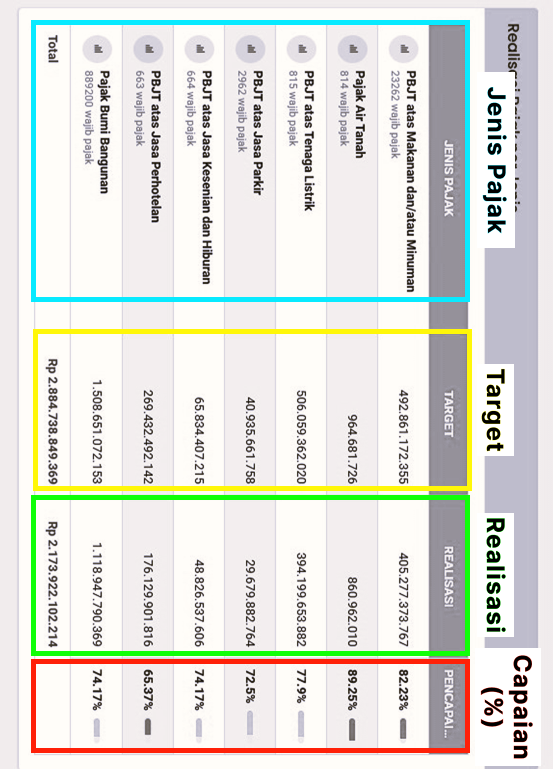
\includegraphics[width=0.76\textwidth]{gambar/wireframe-realisasi-pajak.png}
        \caption{Wireframe Realisasi Pajak}
        \label{fig:wireframe-realisasi-pajak}
    \end{figure}
    \begin{itemize}
        \item \textbf{Fitur Utama:}
            \begin{itemize}
                \item \textbf{Kategorisasi Pajak:} Menampilkan label sektor pajak secara deskriptif (seperti PBJT Makanan, Air Tanah, Tenaga Listrik) untuk mengidentifikasi sumber pendapatan bagi pengguna.
                \item \textbf{Target Finansial:} Menyajikan nominal target penerimaan pajak yang telah ditetapkan dalam periode anggaran tertentu.
                \item \textbf{Realisasi Aktual:} Menampilkan angka riil pendapatan yang telah masuk ke kas daerah berdasarkan transaksi wajib pajak.
                \item \textbf{Indikator Pencapaian:} Berisi perhitungan persentase capaian secara matematis disertai elemen visual berupa \emph{progress bar} berwarna untuk memberikan pemahaman progres secara instan.
            \end{itemize}

        \item \textbf{Analisis Penempatan:}
            \begin{itemize}
                \item \textbf{Penyandingan Horizontal:} Kolom Target dan Realisasi diletakkan berdampingan secara horizontal. Penempatan ini dirancang untuk mempercepat proses kognitif pengguna dalam membandingkan antara sasaran dengan hasil aktual (\emph{plan vs reality}) tanpa perlu memindahkan fokus pandangan terlalu jauh.
                \item \textbf{\emph{Result-Driven Layout}:} Menempatkan kolom Persentase Capaian di posisi paling kanan mengikuti konvensi alur baca manusia dari kiri ke kanan. Hal ini menjadikan kolom tersebut sebagai "titik kesimpulan" atau konklusi dari rincian data finansial yang ada di sebelah kirinya.
                \item \textbf{Efektivitas \emph{Visual Cues}:} Penggunaan \emph{progress bar} berwarnadi akhir kolom memberikan penilaian kinerja secara intuitif. Pengguna dapat langsung mengenali sektor pajak yang memerlukan perhatian khusus melalui visualisasi panjang bar tersebut tanpa harus membaca deretan angka nominal yang panjang, sehingga mendukung prinsip efisiensi operasional sistem \emph{MonPD Reborn}.
            \end{itemize}
    \end{itemize}

\end{itemize}
\section{Implementasi}
\label{sec:implementasi}

Tahap implementasi merupakan proses penerjemahan rancangan arsitektur dan kebutuhan fungsional ke dalam kode program yang berjalan. Pengembangan sistem MonPD Reborn dilakukan dengan menggunakan \emph{framework} ASP.NET Core MVC dan bahasa pemrograman C\#. Penulis berperan penuh dalam pembangunan \emph{Application Layer} (\emph{back-end}) dan \emph{Presentation Layer} (\emph{front-end}) untuk memastikan sistem dapat mengolah data perpajakan dari \emph{database} Oracle secara efisien.

\subsection{Alur Kerja Aplikasi}
\begin{figure}[H]
    \centering
    \begin{tikzpicture}[node distance=1.5cm]
        % Titik Mulai
        \node (start) [startstop] {User Mengakses Menu};
        
        % Tahap 1: Initial Load
        \node (step1) [process, below of=start] {\textbf{1. Pemuatan Kerangka}\\Memuat struktur HTML dasar (\emph{Razor View})};
        
        % Tahap 2: AJAX Request
        \node (step2) [process, below of=step1] {\textbf{2. Permintaan Data}\\Fungsi jQuery memicu \emph{AJAX Request} asinkron};
        
        % Tahap 3: Back-end Processing
        \node (step3) [process, below of=step2] {\textbf{3. Pengolahan Data}\\ \emph{Controller} memanggil \emph{Method} VM $\rightarrow$ Oracle via EF Core};
        
        % Tahap 4: Response
        \node (step4) [process, below of=step3] {\textbf{4. Pengembalian Hasil}\\Server mengirim data (\emph{JSON / Partial View})};
        
        % Tahap 5: Client-side Rendering
        \node (step5) [process, below of=step4] {\textbf{5. Perenderaan Dinamis}\\Data dirender ke DevExtreme DataGrid};

        % Garis Panah
        \draw [arrow] (start) -- (step1);
        \draw [arrow] (step1) -- (step2);
        \draw [arrow] (step2) -- (step3);
        \draw [arrow] (step3) -- (step4);
        \draw [arrow] (step4) -- (step5);
    \end{tikzpicture}
    \caption{Alur Komunikasi Data Asinkron MonPD Reborn}
    \label{fig:web_flow}
\end{figure}

Sistem MonPD Reborn dirancang untuk meminimalkan waktu tunggu pengguna melalui mekanisme pemuatan data asinkron. Berbeda dengan sistem lama yang memuat seluruh data secara sekaligus, alur kerja sistem ini dibagi menjadi beberapa tahapan sebagai berikut:
\begin{enumerate}
    \item \textbf{Pemuatan Kerangka (\emph{Initial Load})}: Saat pengguna mengakses menu, \emph{browser} hanya memuat struktur HTML dasar (\emph{Razor View}) tanpa data. Hal ini membuat halaman terasa instan saat dibuka.
    \item \textbf{Permintaan Data (\emph{AJAX Request})}: Setelah kerangka siap, fungsi JavaScript (jQuery) secara otomatis mengirimkan permintaan ke \emph{Action Method} di \emph{Controller} di latar belakang.
    \item \textbf{Pengolahan Data (\emph{Back-end Processing})}: \emph{Controller} memanggil \emph{method} statis di dalam \emph{ViewModel} yang kemudian bertugas melakukan kueri dan berinteraksi dengan \emph{database} Oracle melalui \emph{Entity Framework Core}.
    \item \textbf{Pengembalian Hasil (\emph{Response})}: Server mengembalikan data hasil olahan tersebut dalam format \emph{Partial View} atau JSON.
    \item \textbf{Perenderaan Dinamis (\emph{Client-side Rendering})}: Komponen DevExtreme DataGrid menerima data tersebut dan menampilkannya kepada pengguna tanpa perlu melakukan penyegaran halaman (\emph{refresh}).
\end{enumerate}

Mekanisme ini memungkinkan halaman terasa instan saat dibuka karena \emph{browser} tidak perlu menunggu seluruh data dari \emph{database} Oracle selesai ditarik sebelum menampilkan antarmuka.

\subsection{Pengembangan \emph{Application Layer} (\emph{Backend})}
Pada proyek ini, diterapkan pola arsitektur \emph{Fat ViewModel} dan \emph{Thin Controller}. Pendekatan ini bertujuan untuk memusatkan seluruh logika bisnis, pemfilteran, dan agregasi data di dalam \emph{ViewModel}, sehingga \emph{Controller} tetap ramping dan hanya berfungsi sebagai pengatur alur permintaan.

\begin{enumerate}
    \item \textbf{Pemetaan Entitas Data (Entity Mapping):} \\
    Sesuai dengan batasan masalah yang memfokuskan pengerjaan pada \emph{Application Layer}, penulis merancang kelas entitas yang merepresentasikan tabel fisik di server Oracle menggunakan \emph{Data Annotations} pada EF Core sebagaimana ditunjukkan pada Kode 4.1.

    \lstinputlisting[language={[Sharp]C}, caption={Pemetaan Entitas C\# ke Tabel Oracle pada Berkas TPemeriksaan.cs}]{program/TPemeriksaan.cs}

    Penjelasan Kode 4.1: Kode ini mendefinisikan hubungan antara properti di dalam kode aplikasi dengan kolom fisik di \emph{database} Bapenda. Penggunaan atribut \texttt{[Table("T\_PEMERIKSAAN")]} dan \texttt{[Column]} memastikan bahwa EF Core dapat melakukan kueri secara akurat ke tabel yang telah dioptimalkan oleh tim \emph{database} Bapenda. Properti dengan tipe data \emph{nullable} seperti \texttt{decimal?} pada \texttt{JumlahKb} digunakan untuk menangani kemungkinan data kosong di \emph{database} tanpa menyebabkan \emph{system crash}.

    \item \textbf{Struktur \emph{ViewModel} dan \emph{Controller}:} 
    Implementasi pola \emph{Thin Controller} ditunjukkan pada Kode 4.2, di mana \\ \texttt{PemeriksaanController} hanya bertugas menerima \emph{request}, melakukan instansiasi \emph{ViewModel}, dan mengembalikan \emph{Partial View}.
    
    \lstinputlisting[language={[Sharp]C}, caption={Implementasi \emph{Thin Controller} pada \texttt{PemeriksaanController.cs}}]{program/PemeriksaanController.cs}

    Penjelasan Kode 4.2: \emph{Action method} \texttt{Detail} menerima parameter \texttt{jenisPajak} dan \texttt{tahun}. Fungsi utama dari kode ini adalah memanggil kelas \emph{ViewModel} \texttt{Detail} dan menangani \emph{error handling} melalui blok \texttt{try-catch} untuk memastikan stabilitas aplikasi jika terjadi kegagalan sistem.

    \item \textbf{Logika Pengambilan Data (Fat ViewModel):} 
    Seluruh logika manipulasi data dipusatkan di dalam \\ \texttt{PemeriksaanVM.cs} seperti yang ditunjukkan pada Kode 4.3.
    
    \lstinputlisting[language={[Sharp]C}, caption={Logika Bisnis pada \emph{Fat ViewModel} \texttt{PemeriksaanVM.cs}}]{program/PemeriksaanVM.cs}

    Penjelasan Kode 4.3: Penulis menggunakan \emph{Entity Framework Core} untuk mengambil data dari tabel \texttt{TPemeriksaan}. Teknik optimasi kunci yang diterapkan adalah penggunaan \texttt{GroupBy} dan \texttt{ToDictionary} untuk melakukan pemetaan data \emph{master} objek pajak di dalam memori (\emph{in-memory mapping}). Hal ini dilakukan untuk menghindari operasi \emph{join} tabel yang berat di sisi \emph{database} Oracle, sehingga proses pencocokan nama Wajib Pajak berdasarkan NOP menjadi jauh lebih cepat.

    \item \textbf{Enkapsulasi Logika:} 
    Seluruh kalkulasi persentase pencapaian dan perbandingan target vs realisasi dilakukan di sisi \emph{server} sebelum dikirim ke \emph{front-end} guna menjaga konsistensi data dan meringankan beban komputasi di sisi \emph{client}.    

    \item \textbf{Implementasi AJAX (\emph{Frontend}):} 
    Untuk mengatasi masalah performa sistem lama, penulis mengimplementasikan fungsi asinkron menggunakan \emph{jQuery} sebagaimana ditunjukkan pada Kode 4.4.
    
    \lstinputlisting[language={JavaScript}, caption={Implementasi AJAX Request pada \texttt{PemeriksaanAJAX.js}}]{program/PemeriksaanAJAX.js}

    Penjelasan Kode 4.4: Fungsi \texttt{loadDetail} mengirimkan data permintaan ke \emph{Controller} di latar belakang. Penggunaan \texttt{beforeSend} berfungsi untuk menampilkan \emph{loading spinner} (\texttt{\#loading2-Detail}) sebagai indikator visual kepada pengguna bahwa data sedang diproses. Setelah data diterima (\emph{success}), hasilnya langsung dirender ke dalam elemen \texttt{\#Detail} tanpa perlu memuat ulang seluruh halaman web. Teknik ini berhasil mereduksi waktu muat secara drastis.
\end{enumerate}

\subsection{Pengembangan \emph{Presentation Layer} (\emph{Frontend})}
Pada \emph{Presentation Layer} (\emph{Frontend}), penulis fokus pada pembangunan antarmuka yang responsif dan interaktif menggunakan jQuery dan \emph{toolkit} DevExtreme.
\begin{enumerate}
    \item \textbf{Implementasi AJAX:} Penulis menulis fungsi \emph{JavaScript} seperti \texttt{fnShow()} untuk memicu pemuatan tabel secara asinkron. Teknik ini berhasil mereduksi waktu muat dari $\pm 120$ detik menjadi hanya $\pm 3 - 5$ detik.
    \item \textbf{Konfigurasi \emph{DevExtreme DataGrid}:} Komponen ini dikonfigurasi untuk menangani volume data besar dengan fitur \emph{server-side paging}. Penulis juga mengimplementasikan \emph{Banded Columns} untuk mengelompokkan data yang berkaitan, seperti kolom ``Pokok'' dan ``Sanksi'' di bawah kategori tahun yang sama.
    \item \textbf{Fitur \emph{Drill-down}:} Melalui fungsi \texttt{showDetailModal()}, pengguna dapat mengklik angka pada tabel rekapitulasi untuk menampilkan \emph{pop-up} detail transaksi individual yang dimuat melalui \emph{Partial View} \texttt{\_Detail.cshtml}.
\end{enumerate}


\subsection{Hasil Implementasi Fitur Utama}
Berikut adalah hasil dari implementasi kode program yang telah dilakukan:
\begin{itemize}
    \item Dashboard Analitik Utama: \\
    Tampilan pusat komando yang menyajikan KPI (\emph{Key Performance Indicator}) secara instan untuk setiap jenis pajak ditunjukkan pada gambar \ref{fig:dashboard-utama-monpd}.
    \begin{figure}[H]
        \centering
        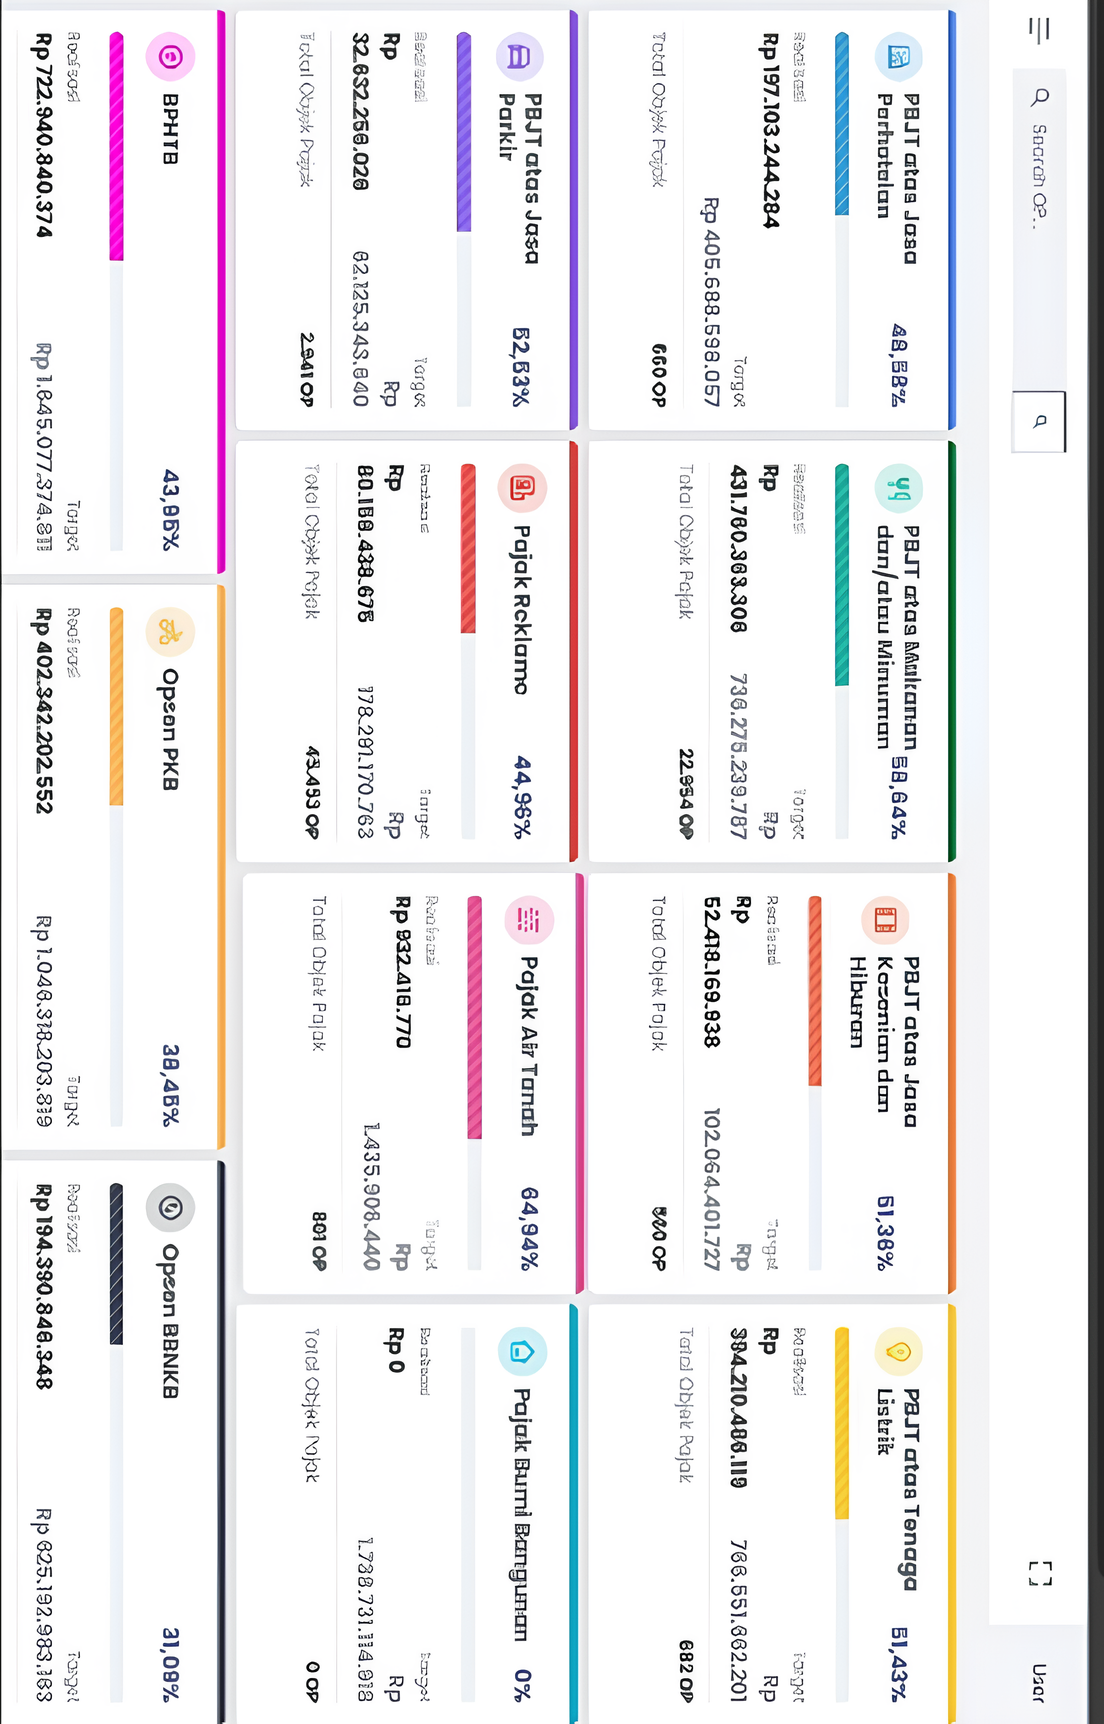
\includegraphics[width=0.95\textwidth]{gambar/dashboard-utama-monpd.png}
        \caption{Tampilan \emph{Dashboard} Utama MonPD Reborn}
        \label{fig:dashboard-utama-monpd}
    \end{figure}

    \item Template Modul Analitik: \\
    Standar tampilan yang memisahkan antara panel filter, ringkasan KPI, dan tabel rincian diimplementasikan pada seluruh modul, seperti yang terlihat pada gambar \ref{fig:dashboard-menu-monpd}.
    \begin{figure}[H]
        \centering
        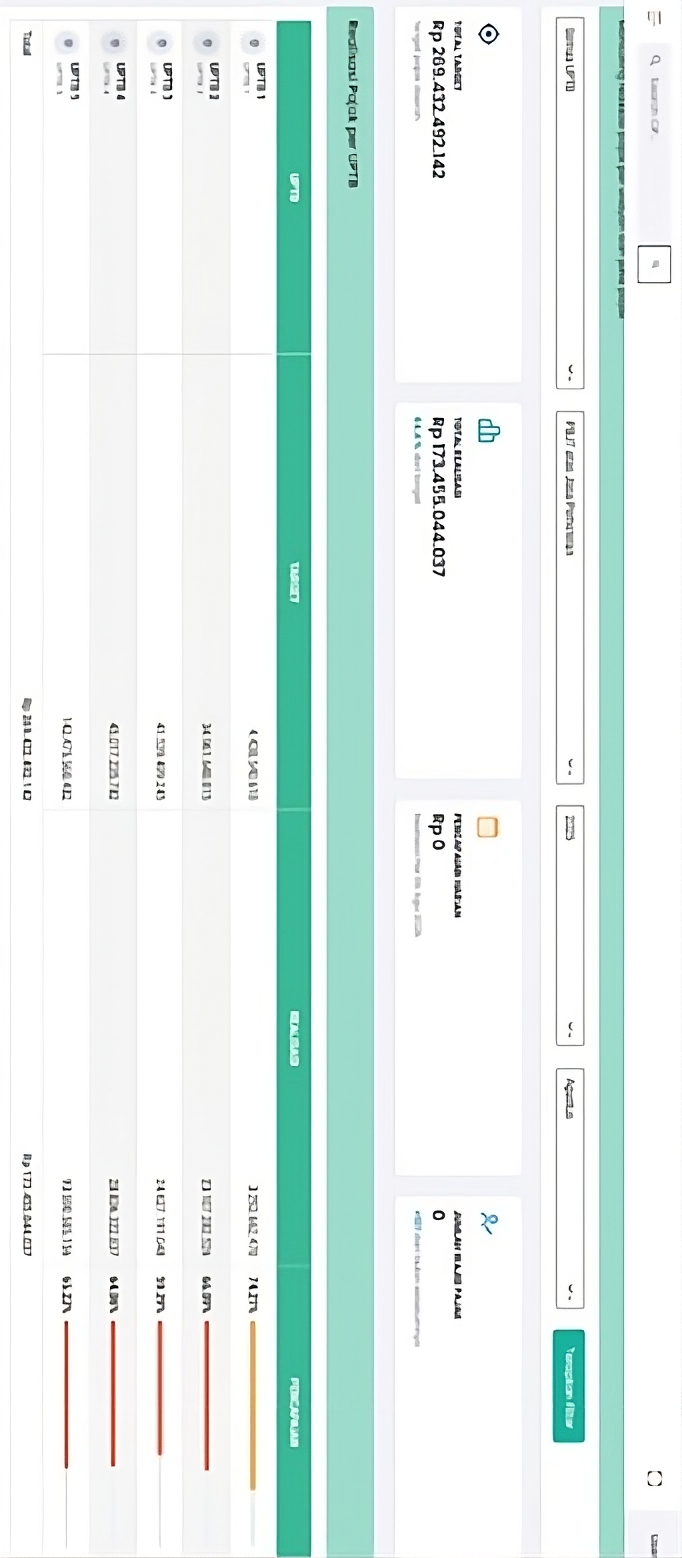
\includegraphics[width=0.55\textwidth]{gambar/dashboard-menu-monpd.png}
        \caption{Tampilan \emph{Dashboard} Menu MonPD Reborn}
        \label{fig:dashboard-menu-monpd}
    \end{figure}

    \item Interaktivitas Data: \\
    Fitur filter per kolom, pencarian instan, dan pengurutan data pada komponen DataGrid ditunjukkan pada gambar \ref{fig:datagrid}.
    \begin{figure}[H]
        \centering
        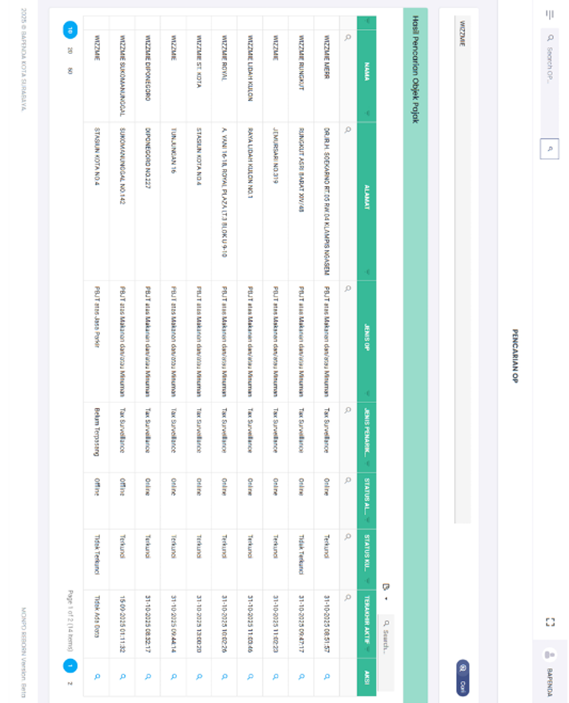
\includegraphics[width=0.99\textwidth]{gambar/datagrid.png}
        \caption{Implementasi DevExtreme DataGrid dengan Fitur Interaktif}
        \label{fig:datagrid}
    \end{figure}

    \item Detail \emph{Pop-up} (\emph{Drill-down}): \\
    Mekanisme pemuatan data detail tanpa kehilangan konteks halaman utama menggunakan modal asinkron ditunjukkan pada gambar \ref{fig:popup-detail}.
    \begin{figure}[H]
        \centering
        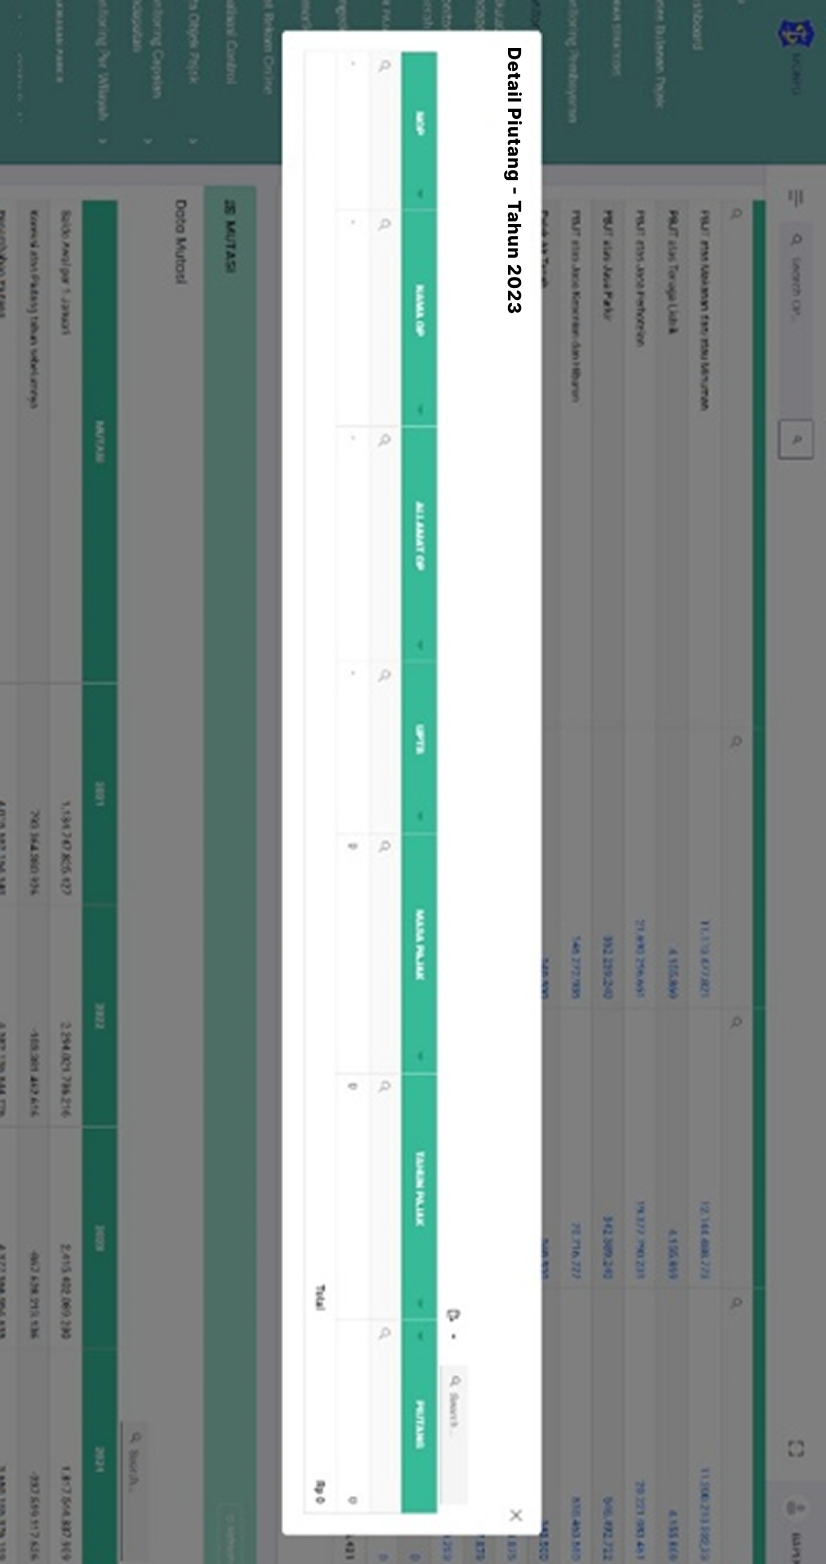
\includegraphics[width=0.67\textwidth]{gambar/popup-detail.png}
        \caption{Implementasi Detail \emph{Pop-up} pada MonPD Reborn}
        \label{fig:popup-detail}
    \end{figure}

    \item Visualisasi Geospasial: \\
    Plot lokasi objek pajak di atas peta Kota Surabaya untuk analisis potensi kewilayahan ditunjukkan pada gambar \ref{fig:geospasial}.
    \begin{figure}[H]
        \centering
        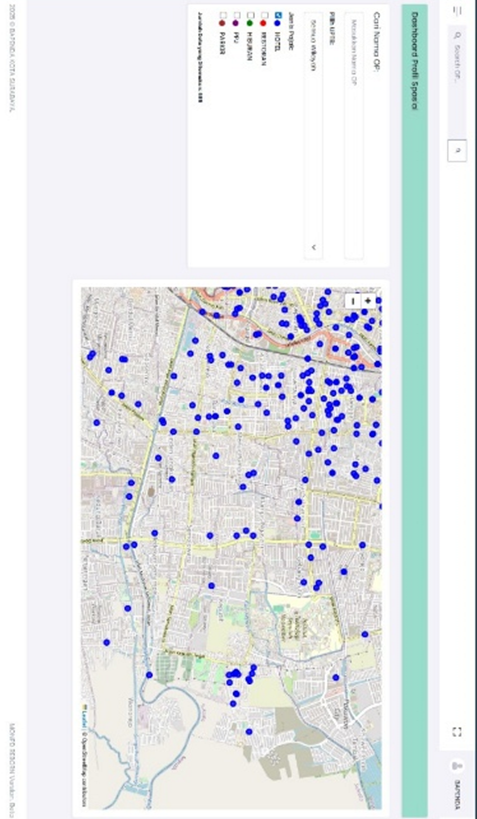
\includegraphics[width=0.76\textwidth]{gambar/geospasial.png}
        \caption{Visualisasi Geospasial pada MonPD Reborn}
        \label{fig:geospasial}
    \end{figure}

    \item Tabel Rekapitulasi Kinerja: \\
    Penyajian perbandingan target dan realisasi yang dilengkapi dengan \emph{progress bar} otomatis ditunjukkan pada gambar \ref{fig:realisasi-pajak}.
    \begin{figure}[H]
        \centering
        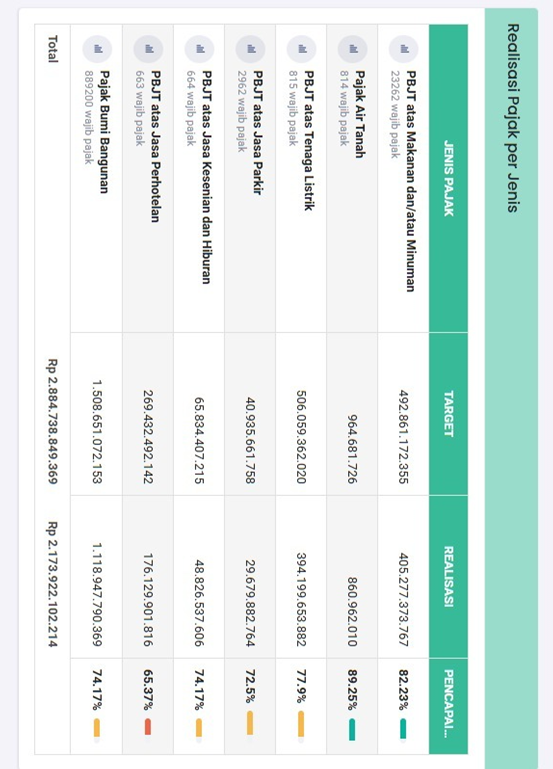
\includegraphics[width=0.93\textwidth]{gambar/realisasi-pajak.png}
        \caption{Tabel Realisasi Pajak}
        \label{fig:realisasi-pajak}
    \end{figure}

\end{itemize}

\section{Hasil dan Dampak Implementasi}
\label{sec:hasildampak}
Implementasi sistem MonPD Reborn berhasil memberikan solusi konkret terhadap tantangan yang dihadapi oleh sistem sebelumnya. Dampak dari pengembangan ini dapat diukur baik secara kualitatif dari pengalaman pengguna maupun secara kuantitatif melalui peningkatan performa dan efisiensi kerja.

\subsection{Peningkatan Performa Sistem}
Salah satu tujuan utama proyek ini adalah mengatasi kelambatan sistem lama. Berdasarkan hasil analisis dan uji coba, tercatat adanya peningkatan performa yang sangat signifikan:
\begin{itemize}
    \item Reduksi Waktu Muat Halaman \\
    Waktu yang dibutuhkan untuk memuat halaman rekap data pada sistem lama dapat mencapai ±120 detik (2 menit) karena seluruh data dimuat secara serentak. Pada sistem MonPD Reborn yang telah dikembangkan, dengan menerapkan teknik \emph{asynchronous loading} (AJAX) dan \emph{server-side paging}, waktu muat rata-rata berhasil direduksi secara drastis menjadi hanya ±3–5 detik.
    \item Peningkatan Kecepatan Lebih dari 95\% \\
    Jika dibandingkan secara langsung, pengurangan waktu muat dari 120 detik menjadi 5 detik ekuivalen dengan peningkatan performa sebesar 95.8\%. Peningkatan ini secara fundamental mengubah pengalaman pengguna dari yang sebelumnya menunggu menjadi nyaris instan.
    \item Efisiensi Transfer Data \\
    Peningkatan kecepatan ini juga disebabkan oleh optimasi \emph{payload} data. Sistem lama mentransfer keseluruhan data set yang bisa berukuran beberapa megabyte dalam satu kali permintaan. Sistem baru, untuk menampilkan halaman pertama sebuah tabel, hanya mentransfer kurang dari 100 KB, karena hanya 10 hingga 20 baris data yang diambil dari total ratusan ribu \emph{record} yang ada di \emph{database}.

\end{itemize}

\subsection{Peningkatan Efisiensi Kerja}
Peningkatan performa teknis secara langsung berdampak pada efisiensi kerja pegawai Bapenda:
\begin{itemize}
    \item Penghematan Waktu Kerja Harian \\
    Dengan eliminasi waktu tunggu yang lama, efisiensi kerja meningkat. Jika seorang pegawai sebelumnya menunggu rata-rata 115 detik untuk setiap halaman yang dibuka dan mengakses sekitar 30 halaman per hari, maka sistem MonPD Reborn berhasil memberikan penghematan waktu tunggu sekitar 57 menit per pegawai setiap harinya. Waktu ini dapat dialokasikan untuk tugas-tugas analisis yang lebih produktif.
    \item Percepatan Analisis Data \\
    Fitur filter, \emph{sorting}, dan pencarian interaktif yang disediakan oleh komponen DevExtreme memungkinkan pengguna untuk mendapatkan data spesifik dalam hitungan detik. Proses yang sebelumnya memerlukan ekspor data ke Excel dan filter manual selama 5-10 menit, kini dapat diselesaikan langsung di aplikasi dalam kurang dari 30 detik.
    \item Pengalaman Pengguna (\emph{User Experience}) yang Lebih Baik \\
    Secara kualitatif, sistem yang responsif dan tidak lambat meningkatkan kepuasan dan mengurangi frustrasi pengguna. Antarmuka yang modern dan intuitif membuat proses monitoring dan analisis data menjadi lebih lancar dan efektif.
\end{itemize}

Dengan demikian, proyek MonPD Reborn tidak hanya berhasil melakukan peremajaan teknologi, tetapi juga memberikan dampak kuantitatif dan kualitatif yang terukur dalam mendukung efisiensi operasional Bapenda Kota Surabaya.


\section{Peran dan Kontribusi Penulis}
\label{sec:perankontribusi}

Pelaksanaan magang di Badan Pendapatan Daerah (Bapenda) Kota Surabaya memberikan ruang bagi penulis untuk berperan aktif dalam seluruh siklus pengembangan sistem \emph{MonPD Reborn}. Sebagai seorang \emph{Full-Stack Developer}, kontribusi penulis tidak hanya terbatas pada pembangunan infrastruktur logika, namun juga mencakup perancangan pengalaman pengguna (\emph{User Experience}) yang bermakna. Penulis berfokus pada transformasi data mentah menjadi informasi yang memiliki nilai analitik (\emph{insightful}), memastikan bahwa setiap elemen visual yang ditampilkan mampu mempermudah pegawai Bapenda dalam melakukan pengolahan dan pengambilan keputusan berbasis data secara instan.

\subsection{Batasan Peran dan Kontribusi}
Selama pelaksanaan proyek Pengembangan Sistem Monitoring Pendapatan Daerah (MonPD Reborn), penulis berperan sebagai \emph{Full-Stack Developer} yang berfokus pada arsitektur \emph{Model} - \emph{View} - \emph{Controller} (MVC) dalam \emph{framework} ASP.NET Core. Kontribusi utama penulis mencakup perancangan dan implementasi di dua lapisan utama: \emph{Presentation Layer} (\emph{Front-End}) dan \emph{Application Layer} (\emph{Back-End}).

\begin{enumerate}
    \item Kontribusi pada \emph{Application Layer} (\emph{Back-End}): \\
    Penulis bertanggung jawab penuh atas seluruh logika bisnis dan alur data di sisi (\emph{Back-End}) aplikasi. Ini mencakup:
    \begin{itemize}
        \item Merancang dan mengimplementasikan arsitektur \emph{Fat ViewModel}, \emph{Thin Controller} menggunakan bahasa C\#.
        \item Membangun kelas-kelas \emph{ViewModel} yang berfungsi sebagai "cetakan" data untuk setiap halaman. Di dalam \emph{method ViewModel} inilah seluruh logika bisnis, pemfilteran, dan agregasi data diimplementasikan.
        \item Membuat \emph{Controller} yang ramping (\emph{thin}) yang hanya bertugas menerima permintaan HTTP dari pengguna dan memanggil \emph{method} yang sesuai di dalam \emph{ViewModel}.
    \end{itemize}

    \item Kontribusi pada \emph{Presentation Layer} (\emph{Front-End}): \\
    Penulis juga bertanggung jawab untuk menerjemahkan rancangan antarmuka (UI/UX) menjadi halaman web yang fungsional, interaktif, dan responsif. Penulis bertanggung jawab untuk mentransformasi rancangan antarmuka menjadi sistem pemantauan yang mampu menyajikan \emph{insight} bagi pengguna. Fokus utama pada lapisan ini adalah memastikan data yang kompleks dapat dibaca secara intuitif untuk kebutuhan analisis strategis. Hal ini mencakup:
    \begin{itemize}
        \item Membangun struktur halaman menggunakan HTML dan \emph{Razor Views} (\texttt{.cshtml}) dengan menerapkan \emph{information hierarchy} agar metrik-metrik penting terlihat lebih menonjol.
        \item Mengimplementasikan seluruh interaktivitas pengguna, terutama fitur pemuatan data asinkron AJAX menggunakan jQuery, yang menjadi solusi utama atas masalah performa sistem.
        \item Mengintegrasikan dan mengkonfigurasi komponen UI canggih dari DevExtreme, seperti DataGrid (untuk \emph{banded columns}, \emph{filtering}, \emph{paging}) dan komponen \emph{dashboard}.
        \item Pembuatan \emph{dashboard} analitik yang memungkinkan pegawai melakukan \emph{drill-down} untuk menemukan anomali atau tren pendapatan secara mandiri.
    \end{itemize}
\end{enumerate}

\subsubsection{Alur Kolaborasi Pengembangan}

Untuk menjamin integritas data dan efisiensi pengembangan, pembagian peran antara tim \emph{database} Bapenda dan penulis diatur melalui alur kerja kolaboratif. Penulis bertanggung jawab penuh pada seluruh proses di sisi aplikasi (\emph{full-stack}), mulai dari pengambilan data hingga perenderaan antarmuka, sebagaimana digambarkan pada Gambar 4.13:

\begin{figure}[H]
    \centering
    \begin{tikzpicture}[node distance=2cm, transform shape, scale=0.9]
        % Porsi Tim Database
        \node (db1) [dbteam] {\textbf{Tim Database Bapenda (Oracle Server)}\\Penyediaan \emph{Stored Procedures} atau \emph{Query} yang tervalidasi dan optimal};
        
        % Porsi Penulis (Warna berbeda)
        \node (auth1) [author, below of=db1] {\textbf{Penulis (Application Layer)}\\Pemanggilan fungsi/\emph{Stored Procedure} melalui kode C\# menggunakan EF Core};
        \node (auth2) [author, below of=auth1] {\textbf{Penulis (ViewModel)}\\Pengolahan, manipulasi, dan \emph{formatting} data agar siap dikonsumsi \emph{View}};
        \node (auth3) [author, below of=auth2] {\textbf{Penulis (Presentation Layer)}\\Perenderaan data secara dinamis ke dalam \emph{View} (\texttt{.cshtml}) menggunakan \emph{DevExtreme}};

        % Garis Panah
        \draw [arrow] (db1) -- (auth1);
        \draw [arrow] (auth1) -- (auth2);
        \draw [arrow] (auth2) -- (auth3);
    \end{tikzpicture}
    \caption{Alur Kolaborasi dan Batasan Kontribusi Penulis}
    \label{fig:alur_kolaborasi}
\end{figure}

Berdasarkan alur di atas, kontribusi penulis tidak hanya terbatas pada \emph{Application Layer} (pengolahan logika di \emph{ViewModel}), tetapi mencakup seluruh siklus penyajian data di \emph{Presentation Layer}. Hal ini meliputi penulisan skrip \emph{JavaScript/jQuery} untuk pengambilan data asinkron hingga memastikan komponen DevExtreme menampilkan data secara akurat di sisi pengguna (\emph{client-side}).

Secara ringkas, peran penulis adalah sebagai jembatan utama yang mengubah kompleksitas data di server Oracle menjadi antarmuka analitik yang interaktif. Penulis memastikan bahwa setiap fitur yang dikembangkan tidak hanya berfungsi secara teknis, tetapi juga memberikan kemudahan operasional bagi pegawai Bapenda dalam mengawal optimalisasi pendapatan daerah.
  \cleardoublepage

  % Bab 5 
  \chapter{PENUTUP}
\label{chap:penutup}

% Ubah bagian-bagian berikut dengan isi dari penutup
\section{Kesimpulan}
\label{sec:kesimpulan}

Berdasarkan keseluruhan proses magang dan pengembangan sistem, dapat disimpulkan bahwa proyek "Pengembangan Sistem Monitoring Pendapatan Daerah (MonPD Reborn) Berbasis .NET" telah berhasil diselesaikan dan secara efektif menjawab permasalahan utama yang dihadapi oleh sistem sebelumnya. Proyek ini sukses menghasilkan serangkaian modul fungsional yang tidak hanya menyajikan data secara interaktif, tetapi juga secara fundamental memperbaiki masalah performa sistem yang sebelumnya menjadi kendala operasional utama.

Keberhasilan utama dari proyek ini adalah implementasi arsitektur aplikasi modern menggunakan ASP.NET Core MVC yang menerapkan teknik pemuatan data secara asinkron (AJAX). Secara kuantitatif, sistem MonPD Reborn berhasil mereduksi waktu muat halaman rata-rata dari $\pm120$ detik pada sistem lama menjadi hanya $3-5$ detik, yang merepresentasikan peningkatan performa sebesar 95.8\%. Selain itu, optimasi pengiriman data berhasil menekan besaran \textit{payload} dari satuan megabyte menjadi kurang dari 100 KB per \emph{request}. Dengan pendekatan ini, aplikasi berhasil mengatasi masalah kelambatan karena data hanya dimuat sesuai kebutuhan pengguna dan tidak lagi membebani \textit{server} maupun \textit{browser} saat pertama kali diakses.

Implementasi fitur pemantauan dan analisis yang dikembangkan telah menyediakan alat yang andal bagi Bapenda untuk meningkatkan pengawasan pendapatan daerah. Dampak operasional yang dihasilkan sangat signifikan, dengan estimasi penghematan waktu kerja rata-rata sebesar $\pm57$ menit per hari bagi setiap pegawai pengguna sistem. Dengan demikian, proyek ini tidak hanya menjadi penerapan ilmu teknis rekayasa perangkat lunak, tetapi juga sebuah solusi konkret yang berhasil meningkatkan efisiensi operasional dan performa teknologi informasi di lingkungan kerja Bapenda Kota Surabaya.
\section{Saran}
\label{sec:saran}

Meskipun sistem yang dikembangkan telah memenuhi kebutuhan awal, terdapat beberapa aspek yang dapat menjadi fokus untuk pengembangan di masa mendatang guna menyempurnakan fungsionalitas dan nilai tambah aplikasi.
\begin{itemize}
    \item Pengembangan Hak Akses Berjenjang: Disarankan untuk mengimplementasikan sistem otorisasi dan hak akses yang lebih granular. Misalnya, membatasi akses data UPTB hanya untuk pegawai dari UPTB yang bersangkutan, sementara pimpinan memiliki akses ke seluruh data.
    \item Sistem Notifikasi Otomatis: Mengembangkan fitur notifikasi (misalnya, via email atau dashboard alert) untuk memberitahu pengguna tentang kejadian penting, seperti adanya surat penagihan yang akan jatuh tempo atau data pemeriksaan baru yang perlu divalidasi, dapat meningkatkan proaktivitas pengguna.
\end{itemize}
  \cleardoublepage

  % Daftar pustaka
  \renewcommand\bibname{DAFTAR PUSTAKA}
  \addcontentsline{toc}{chapter}{\bibname}
  \bibliographystyle{unsrtnat}
  \bibliography{pustaka/pustaka.bib}
  \cleardoublepage

  % Biografi penulis
  \begin{center}
  \Large\textbf{BIOGRAFI PENULIS}
\end{center}
\vspace{2ex}

\addcontentsline{toc}{chapter}{BIOGRAFI PENULIS}

% Ubah kalimat berikut dengan biografi dari mahasiswa pertama
\noindent Elon Reeve Musk, lahir pada \lipsum[1]

\vspace{2ex}

% Ubah kalimat berikut dengan biografi dari mahasiswa kedua
\noindent Felix Arvid Ulf Kjellberg, lahir pada \lipsum[2]

  \cleardoublepage

\end{document}
